% Options for packages loaded elsewhere
\PassOptionsToPackage{unicode}{hyperref}
\PassOptionsToPackage{hyphens}{url}
%
\documentclass[
]{book}
\usepackage{lmodern}
\usepackage{amssymb,amsmath}
\usepackage{ifxetex,ifluatex}
\ifnum 0\ifxetex 1\fi\ifluatex 1\fi=0 % if pdftex
  \usepackage[T1]{fontenc}
  \usepackage[utf8]{inputenc}
  \usepackage{textcomp} % provide euro and other symbols
\else % if luatex or xetex
  \usepackage{unicode-math}
  \defaultfontfeatures{Scale=MatchLowercase}
  \defaultfontfeatures[\rmfamily]{Ligatures=TeX,Scale=1}
\fi
% Use upquote if available, for straight quotes in verbatim environments
\IfFileExists{upquote.sty}{\usepackage{upquote}}{}
\IfFileExists{microtype.sty}{% use microtype if available
  \usepackage[]{microtype}
  \UseMicrotypeSet[protrusion]{basicmath} % disable protrusion for tt fonts
}{}
\makeatletter
\@ifundefined{KOMAClassName}{% if non-KOMA class
  \IfFileExists{parskip.sty}{%
    \usepackage{parskip}
  }{% else
    \setlength{\parindent}{0pt}
    \setlength{\parskip}{6pt plus 2pt minus 1pt}}
}{% if KOMA class
  \KOMAoptions{parskip=half}}
\makeatother
\usepackage{xcolor}
\IfFileExists{xurl.sty}{\usepackage{xurl}}{} % add URL line breaks if available
\IfFileExists{bookmark.sty}{\usepackage{bookmark}}{\usepackage{hyperref}}
\hypersetup{
  pdftitle={Técnicas cuantitativas},
  pdfauthor={Enric Aguilar y Benito Zaragozí},
  hidelinks,
  pdfcreator={LaTeX via pandoc}}
\urlstyle{same} % disable monospaced font for URLs
\usepackage{color}
\usepackage{fancyvrb}
\newcommand{\VerbBar}{|}
\newcommand{\VERB}{\Verb[commandchars=\\\{\}]}
\DefineVerbatimEnvironment{Highlighting}{Verbatim}{commandchars=\\\{\}}
% Add ',fontsize=\small' for more characters per line
\usepackage{framed}
\definecolor{shadecolor}{RGB}{248,248,248}
\newenvironment{Shaded}{\begin{snugshade}}{\end{snugshade}}
\newcommand{\AlertTok}[1]{\textcolor[rgb]{0.94,0.16,0.16}{#1}}
\newcommand{\AnnotationTok}[1]{\textcolor[rgb]{0.56,0.35,0.01}{\textbf{\textit{#1}}}}
\newcommand{\AttributeTok}[1]{\textcolor[rgb]{0.77,0.63,0.00}{#1}}
\newcommand{\BaseNTok}[1]{\textcolor[rgb]{0.00,0.00,0.81}{#1}}
\newcommand{\BuiltInTok}[1]{#1}
\newcommand{\CharTok}[1]{\textcolor[rgb]{0.31,0.60,0.02}{#1}}
\newcommand{\CommentTok}[1]{\textcolor[rgb]{0.56,0.35,0.01}{\textit{#1}}}
\newcommand{\CommentVarTok}[1]{\textcolor[rgb]{0.56,0.35,0.01}{\textbf{\textit{#1}}}}
\newcommand{\ConstantTok}[1]{\textcolor[rgb]{0.00,0.00,0.00}{#1}}
\newcommand{\ControlFlowTok}[1]{\textcolor[rgb]{0.13,0.29,0.53}{\textbf{#1}}}
\newcommand{\DataTypeTok}[1]{\textcolor[rgb]{0.13,0.29,0.53}{#1}}
\newcommand{\DecValTok}[1]{\textcolor[rgb]{0.00,0.00,0.81}{#1}}
\newcommand{\DocumentationTok}[1]{\textcolor[rgb]{0.56,0.35,0.01}{\textbf{\textit{#1}}}}
\newcommand{\ErrorTok}[1]{\textcolor[rgb]{0.64,0.00,0.00}{\textbf{#1}}}
\newcommand{\ExtensionTok}[1]{#1}
\newcommand{\FloatTok}[1]{\textcolor[rgb]{0.00,0.00,0.81}{#1}}
\newcommand{\FunctionTok}[1]{\textcolor[rgb]{0.00,0.00,0.00}{#1}}
\newcommand{\ImportTok}[1]{#1}
\newcommand{\InformationTok}[1]{\textcolor[rgb]{0.56,0.35,0.01}{\textbf{\textit{#1}}}}
\newcommand{\KeywordTok}[1]{\textcolor[rgb]{0.13,0.29,0.53}{\textbf{#1}}}
\newcommand{\NormalTok}[1]{#1}
\newcommand{\OperatorTok}[1]{\textcolor[rgb]{0.81,0.36,0.00}{\textbf{#1}}}
\newcommand{\OtherTok}[1]{\textcolor[rgb]{0.56,0.35,0.01}{#1}}
\newcommand{\PreprocessorTok}[1]{\textcolor[rgb]{0.56,0.35,0.01}{\textit{#1}}}
\newcommand{\RegionMarkerTok}[1]{#1}
\newcommand{\SpecialCharTok}[1]{\textcolor[rgb]{0.00,0.00,0.00}{#1}}
\newcommand{\SpecialStringTok}[1]{\textcolor[rgb]{0.31,0.60,0.02}{#1}}
\newcommand{\StringTok}[1]{\textcolor[rgb]{0.31,0.60,0.02}{#1}}
\newcommand{\VariableTok}[1]{\textcolor[rgb]{0.00,0.00,0.00}{#1}}
\newcommand{\VerbatimStringTok}[1]{\textcolor[rgb]{0.31,0.60,0.02}{#1}}
\newcommand{\WarningTok}[1]{\textcolor[rgb]{0.56,0.35,0.01}{\textbf{\textit{#1}}}}
\usepackage{longtable,booktabs}
% Correct order of tables after \paragraph or \subparagraph
\usepackage{etoolbox}
\makeatletter
\patchcmd\longtable{\par}{\if@noskipsec\mbox{}\fi\par}{}{}
\makeatother
% Allow footnotes in longtable head/foot
\IfFileExists{footnotehyper.sty}{\usepackage{footnotehyper}}{\usepackage{footnote}}
\makesavenoteenv{longtable}
\usepackage{graphicx,grffile}
\makeatletter
\def\maxwidth{\ifdim\Gin@nat@width>\linewidth\linewidth\else\Gin@nat@width\fi}
\def\maxheight{\ifdim\Gin@nat@height>\textheight\textheight\else\Gin@nat@height\fi}
\makeatother
% Scale images if necessary, so that they will not overflow the page
% margins by default, and it is still possible to overwrite the defaults
% using explicit options in \includegraphics[width, height, ...]{}
\setkeys{Gin}{width=\maxwidth,height=\maxheight,keepaspectratio}
% Set default figure placement to htbp
\makeatletter
\def\fps@figure{htbp}
\makeatother
\setlength{\emergencystretch}{3em} % prevent overfull lines
\providecommand{\tightlist}{%
  \setlength{\itemsep}{0pt}\setlength{\parskip}{0pt}}
\setcounter{secnumdepth}{5}
\usepackage{booktabs}

\ifxetex
  \usepackage{polyglossia}
  \setmainlanguage{spanish}
  % Tabla en lugar de cuadro
  \gappto\captionsspanish{\renewcommand{\tablename}{Tabla}  
          \renewcommand{\listtablename}{Índice de tablas}}
\else
  \usepackage[spanish,es-tabla]{babel}
\fi
\usepackage[]{natbib}
\bibliographystyle{apalike}

\title{Técnicas cuantitativas}
\author{Enric Aguilar y Benito Zaragozí}
\date{19-Mar-2021}

\begin{document}
\maketitle

{
\setcounter{tocdepth}{1}
\tableofcontents
}
\hypertarget{antes-de-empezar}{%
\chapter{Antes de empezar}\label{antes-de-empezar}}

En este breve capítulo explicamos los aspectos básicos para que podáis reproducir los ejercicios y entregar las actividades utilizando Markdown y Rstudio. Aquí planteamos los conceptos básicos para preparar un documento que incluye explicaciónes, código y los resultados de análisis R. Se trata de una estratégia de \textbf{\emph{programación literaria}} que en los últimos años está siendo cada vez más utilizada en el análisis de datos \citep{knuth1984literate, xie2015knitr}.

\hypertarget{prerrequisitos}{%
\section{Prerrequisitos}\label{prerrequisitos}}

Para preparar cualquier tarea en este formato es necesario instalar primero R y RStudio con los paquetes \texttt{knitr} y \texttt{rmarkdown}.

\hypertarget{tipos-de-ficheros}{%
\section{Tipos de ficheros}\label{tipos-de-ficheros}}

\begin{itemize}
\tightlist
\item
  Los archivos para producir documentos de RMarkdown tienen la extensión \texttt{.Rmd}.
\item
  Los archivos deben abrirse con RStudio y se compilan haciendo clic en el botón knitr.
\item
  El resultado es un documento en formato \texttt{.pdf}, \texttt{.html} o \texttt{.doc}.
\end{itemize}

\hypertarget{un-ejemplo-muy-sencillo}{%
\section{Un ejemplo muy sencillo}\label{un-ejemplo-muy-sencillo}}

Cread un fichero con el siguiente contenido

\begin{verbatim}
Hola, soy **R Markdown**

Aprende más sobre mi [aquí](http://rmarkdown.rstudio.com/).
\end{verbatim}

al hacer clic en el botón \texttt{knitr\ a\ HTML} de Rstudio se crea un archivo \texttt{.html} con este contenido.

\hypertarget{estructura-buxe1sica-de-un-documento-markdown}{%
\section{Estructura básica de un documento Markdown}\label{estructura-buxe1sica-de-un-documento-markdown}}

Revisemos las partes más importantes del documento \texttt{Rmd}.

\hypertarget{cabecera}{%
\subsection{Cabecera}\label{cabecera}}

La cabecera está en la parte superior del documento dentro de estas dos líneas \texttt{-\/-\/-}

\begin{verbatim}
---
title: "Write your title here"
author: "Write your name here"
date: "Write the date here"
output:
  pdf_document: default
  html_document: default
  word_document: default
---
\end{verbatim}

En el encabezado del archivo debe escribir el título del documento, su nombre y la fecha. La declaración de salida se utiliza para la clase del documento final, \texttt{pdf}, \texttt{html}o \texttt{doc}. Para producir un PDF es necesario tener instalado un motor de LaTeX.

\hypertarget{insertar-cuxf3digo-r}{%
\subsection{Insertar código R}\label{insertar-cuxf3digo-r}}

A continuación, configuramos las opciones necesarias para imprimir el código R y la salida R en el documento final.

La primera línea es ocultar este fragmento de código en el documento final.

La segunda línea es para imprimir el código R y la salida R en el documento final.

\hypertarget{formatos-de-texto}{%
\subsection{Formatos de texto}\label{formatos-de-texto}}

El texto sin formato se escribe como en cualquier otro documento, como un documento de Word. Debe tener cuidado con las letras en cursiva o negrita y algunos caracteres especiales. Por ejemplo

\begin{itemize}
\tightlist
\item
  \textbf{Negrita}: escriba el texto entre **Negrita** o \_\_Negrita\_\_
\item
  \emph{Cursiva}: escriba su texto entre*cursiva* o \_Italica\_
\item
  Encabezados de sección
\end{itemize}

\begin{verbatim}
# Título 1
## Título 2
### Título 3
\end{verbatim}

Cuantos más símbolos \# escriba antes de su texto, menor será el tamaño de su título

Puede encontrar más información sobre cómo escribir en el siguiente \href{https://rstudio.com/wp-content/uploads/2015/02/rmarkdown-cheatsheet.pdf}{archivo}.

\hypertarget{generando-el-documento}{%
\subsection{Generando el documento}\label{generando-el-documento}}

Para compilar el archivo \texttt{.Rmd} y obtener su documento final, simplemente haga clic en el botón \texttt{Knit} y seleccione \texttt{Knit\ a\ PDF} para producir un archivo \texttt{.pdf}.

\hypertarget{intro}{%
\chapter{Introducción a R}\label{intro}}

\hypertarget{r-como-lenguaje-de-programaciuxf3n}{%
\section{R como lenguaje de programación}\label{r-como-lenguaje-de-programaciuxf3n}}

\textbf{\href{https://www.r-project.org/}{R}} fue creado en 1992 por Ross Ihaka y Robert Gentleman en la Universidad de Auckland, Nueva Zelanda. R es una implementación gratuita de código abierto del lenguaje de programación estadística \textbf{S} creado inicialmente en Bell Labs. En esencia, R es un lenguaje de programación funcional (sus principales funcionalidades giran en torno a la definición y ejecución de funciones). Sin embargo, ahora es compatible, y se usa comúnmente como un lenguaje de programación imperativo (enfocado en instrucciones sobre variables y estructuras de control de programación) y orientado a objetos (que involucra estructuras de objetos complejas).

En términos simples, hoy en día, la programación en R se enfoca principalmente en diseñar una serie de instrucciones para ejecutar una tarea, más comúnmente, cargar y analizar un conjunto de datos.

Como tal, R se puede usar para programar creando secuencias de \textbf{instrucciones} que involucren \textbf{variables}, que son entidades con nombre que pueden almacenar valores. Ese será el tema principal de esta sesión práctica. Las instrucciones pueden incluir estructuras de flujo de control, como puntos de decisión (\emph{if/else}) y bucles, que serán el tema de la próxima sesión práctica. Las instrucciones también se pueden agrupar en \textbf{funciones}, que también veremos en la próxima sesión práctica.

R es \textbf{interpretado}, no compilado. Lo que significa que un intérprete de R (si está utilizando R Studio, el intérprete de R simplemente está oculto en el backend y R Studio es el frontend que le permite interactuar con el intérprete) recibe una instrucción que escribe en R, la interpreta y la ejecuta . Otros lenguajes de programación requieren que su código sea compilado en un ejecutable para ser ejecutado en un ordenador.

\hypertarget{utilizando-rstudio}{%
\section{Utilizando RStudio}\label{utilizando-rstudio}}

La interfaz de RStudio se divide en dos secciones principales. En el lado izquierdo, encontrará la \emph{Consola}, así como el editor de secuencias de comandos R, cuando se está editando una secuencia de comandos. La \emph{Consola} en una ventana de entrada/salida en el intérprete de R, donde se pueden escribir instrucciones y se muestra la salida calculada.

Por ejemplo, si escribís en la \emph{Consola}

\begin{Shaded}
\begin{Highlighting}[]
\DecValTok{1} \OperatorTok{+}\StringTok{ }\DecValTok{1}
\end{Highlighting}
\end{Shaded}

el intérprete de R entiende eso como una instrucción para sumar uno más uno, y produce el resultado (dado que los materiales para este módulo se crean en RMarkdown, la salida del cálculo siempre está precedida por `\#\#').

\begin{verbatim}
## [1] 2
\end{verbatim}

Fíjate cómo el valor de salida \texttt{2} está precedido por \texttt{{[}1{]}}, lo que indica que la salida está constituida por un solo elemento. Si la salida está constituida por más de un elemento, como la lista de números a continuación, cada fila de la salida está precedida por el índice del primer elemento de la salida.

\begin{verbatim}
##  [1]   1   4   9  16  25  36  49  64  81 100 121 144 169 196 225 256 289 324 361
## [20] 400
\end{verbatim}

En el lado derecho, encontrarás dos grupos de paneles. En la parte superior derecha, el elemento principal es el panel \emph{Entorno}, que es una representación del estado actual de la memoria del intérprete y, como tal, muestra todas las variables, conjuntos de datos y funciones almacenados. En la parte inferior derecha, encontrarás el panel \emph{Archivos}, que muestra el sistema de archivos (archivos y carpetas del ordenador), así como el panel \emph{Ayuda}, que le muestra las páginas de ayuda cuando sea necesario. Discutiremos los otros paneles más adelante.

\hypertarget{interpretaciuxf3n-de-valores}{%
\section{Interpretación de valores}\label{interpretaciuxf3n-de-valores}}

Cuando se escribe un valor en la \emph{Consola}, el intérprete simplemente devuelve el mismo valor. En los ejemplos siguientes, \texttt{2} es un valor numérico simple, mientras que \texttt{"Valor\ de\ cadena"} es un valor textual, que en R se conoce como un valor de \emph{carácter} y en programación también se conoce comúnmente como una \emph{cadena} (abreviatura de \emph{una cadena de caracteres}).

Ejemplo númerico

\begin{Shaded}
\begin{Highlighting}[]
\DecValTok{2}
\end{Highlighting}
\end{Shaded}

\begin{verbatim}
## [1] 2
\end{verbatim}

Ejemplo de cadena

\begin{Shaded}
\begin{Highlighting}[]
\StringTok{"String value"}
\end{Highlighting}
\end{Shaded}

\begin{verbatim}
## [1] "String value"
\end{verbatim}

Tened en cuenta que los valores de los caracteres deben comenzar y terminar con comillas simples o dobles (\texttt{\textquotesingle{}}o\texttt{"}), que no forman parte de la información en sí. La \href{https://style.tidyverse.org\%20/syntax.html}{Guía de estilo de Tidyverse} sugiere usar siempre comillas dobles (\texttt{"}), así que serán las que usaremos en este curso.

Todo lo que sigue a un símbolo \texttt{\#} se considera un \emph{comentario} y el intérprete lo ignora. Cada lenguaje de programación puede usar sus propios símbolos para identificar los comentarios. Por ejemplo cabe destacar la diferencia entre \texttt{\#} en Markdown que identifica un título de primer nivel, mientras que los comentarios en un fichero de Rmarkdown se identifican entre \texttt{\textless{}} y \texttt{\textgreater{}}.

\begin{Shaded}
\begin{Highlighting}[]
\CommentTok{# Este comentario es ignorado por R. Solo sirve para documentar el código.}
\end{Highlighting}
\end{Shaded}

Como se ha mencionado anteriormente, el intérprete también comprende \href{https://stat.ethz.ch/R-manual/R-devel/library/base/html/Arithmetic.html}{operaciones aritméticas simples sobre valores numéricos}.

\begin{Shaded}
\begin{Highlighting}[]
\DecValTok{1} \OperatorTok{+}\StringTok{ }\DecValTok{1}
\end{Highlighting}
\end{Shaded}

\begin{verbatim}
## [1] 2
\end{verbatim}

Además, también hay una gran cantidad de funciones predefinidas, por ejemplo, raíz cuadrada: \texttt{sqrt}.

\begin{Shaded}
\begin{Highlighting}[]
\KeywordTok{sqrt}\NormalTok{(}\DecValTok{2}\NormalTok{)}
\end{Highlighting}
\end{Shaded}

\begin{verbatim}
## [1] 1.414214
\end{verbatim}

Las funciones se recopilan y almacenan en \emph{bibliotecas} (a veces denominadas \emph{paquetes}), que contienen funciones relacionadas. Las bibliotecas pueden variar desde la biblioteca \texttt{base}, que incluye la función \texttt{sqrt} anterior, hasta la biblioteca \texttt{rgdal}, que funciona como un puente hacia las funciones de la \href{https://gdal.org/}{GDAL (Biblioteca de abstracción de datos geoespaciales)}, que es una importante librería en el mundo de los Sistemas de Información Geográfica. Por lo tanto, es mediante la creación de librerías que podemos extender las capacidades de R.

\hypertarget{variables}{%
\section{Variables}\label{variables}}

Una variable se puede definir usando un \textbf{identificador} (por ejemplo, \texttt{una\_variable}) a la izquierda de un \textbf{operador de asignación} \texttt{\textless{}-}, seguido del \emph{objeto} que se vinculará al identificador, como un \textbf{valor} (por ejemplo, \texttt{1}) que se asignará a la derecha. Una vez realizada la asignación, el valor de la variable se puede probar/invocar simplemente especificando el \textbf{identificador}.

\begin{Shaded}
\begin{Highlighting}[]
\NormalTok{una_variable <-}\StringTok{ }\DecValTok{1}
\NormalTok{una_variable}
\end{Highlighting}
\end{Shaded}

\begin{verbatim}
## [1] 1
\end{verbatim}

Si escribes \texttt{una\_variable\ \textless{}-\ 1} en la \emph{Consola} de RStudio, aparece un nuevo elemento en el panel \emph{Environment} (derecha-arriba), que representa la nueva variable en la memoria. La parte izquierda de la entrada contiene el identificador \texttt{una\_variable}, y la parte derecha contiene el valor asignado a la variable\texttt{una\_variable}, es decir, \texttt{1}.

No es necesario aportar un valor directamente. La parte derecha de la tarea puede ser una \textbf{llamada a una función}. En ese caso, la función se \textbf{ejecuta} en la entrada proporcionada y \textbf{el resultado se asigna a la variable}.

\begin{Shaded}
\begin{Highlighting}[]
\NormalTok{una_variable <-}\StringTok{ }\KeywordTok{sqrt}\NormalTok{(}\DecValTok{4}\NormalTok{)}
\NormalTok{una_variable}
\end{Highlighting}
\end{Shaded}

\begin{verbatim}
## [1] 2
\end{verbatim}

Observa cómo, al escribir \texttt{una\_variable\ \textless{}-\ sqrt\ (4)} en la \emph{Consola} de RStudio, el elemento en el panel \emph{Environment} cambia para reflejar el nuevo valor asignado a \texttt{una\_variable}, que ahora es el resultado de \texttt{sqrt\ (4)}, es decir 2.

En el siguiente ejemplo, se crea otra variable llamada \texttt{otra\_variable} y se suma a \texttt{una\_variable}, guardando el resultado en \texttt{suma\_de\_dos\_variables}. La raíz cuadrada de esa suma se almacena en la variable \texttt{raiz\_cuadrada\_de\_suma}.

\begin{Shaded}
\begin{Highlighting}[]
\NormalTok{otra_variable <-}\StringTok{ }\DecValTok{4}
\NormalTok{otra_variable}
\end{Highlighting}
\end{Shaded}

\begin{verbatim}
## [1] 4
\end{verbatim}

\begin{Shaded}
\begin{Highlighting}[]
\NormalTok{suma_de_dos_variables <-}\StringTok{ }\NormalTok{una_variable }\OperatorTok{+}\StringTok{ }\NormalTok{otra_variable}

\NormalTok{raiz_cuadrada_de_suma <-}\StringTok{ }\KeywordTok{sqrt}\NormalTok{(suma_de_dos_variables)}
\NormalTok{raiz_cuadrada_de_suma}
\end{Highlighting}
\end{Shaded}

\begin{verbatim}
## [1] 2.44949
\end{verbatim}

\hypertarget{tipos-basicos}{%
\section{Tipos basicos}\label{tipos-basicos}}

\hypertarget{nuxfameros}{%
\subsection{Números}\label{nuxfameros}}

El tipo \emph{numeric} representa números en general (tanto enteros como reales), pero R es capaz de distinguirlos utilizando funciones.

\begin{Shaded}
\begin{Highlighting}[]
\NormalTok{un_numero <-}\StringTok{ }\FloatTok{1.41}
\KeywordTok{is.numeric}\NormalTok{(un_numero)}
\end{Highlighting}
\end{Shaded}

\begin{verbatim}
## [1] TRUE
\end{verbatim}

\begin{Shaded}
\begin{Highlighting}[]
\KeywordTok{is.integer}\NormalTok{(un_numero)}
\end{Highlighting}
\end{Shaded}

\begin{verbatim}
## [1] FALSE
\end{verbatim}

\begin{Shaded}
\begin{Highlighting}[]
\KeywordTok{is.double}\NormalTok{(un_numero) }\CommentTok{# i.e., es real}
\end{Highlighting}
\end{Shaded}

\begin{verbatim}
## [1] TRUE
\end{verbatim}

Operadores numéricos básicos.

\begin{longtable}[]{@{}llll@{}}
\toprule
Operador & Significado & Ejemplo & Resultado\tabularnewline
\midrule
\endhead
+ & Suma & \texttt{5+2} & 7\tabularnewline
- & Resta & \texttt{5-2} & 3\tabularnewline
\texttt{*} & Multiplicación & \texttt{5*2} & 10\tabularnewline
/ & División & \texttt{5/2} & 2.5\tabularnewline
\%/\% & Div. de enteros & \texttt{5\%/\%2} & 2\tabularnewline
\%\% & Módulo & \texttt{5\%\%2} & 1\tabularnewline
\^{} & Potencia & \texttt{5\^{}2} & 25\tabularnewline
\bottomrule
\end{longtable}

Algunas funciones predefinidas en R son:

\begin{Shaded}
\begin{Highlighting}[]
\KeywordTok{abs}\NormalTok{(}\OperatorTok{-}\DecValTok{2}\NormalTok{) }\CommentTok{# Valor absoluto}
\end{Highlighting}
\end{Shaded}

\begin{verbatim}
## [1] 2
\end{verbatim}

\begin{Shaded}
\begin{Highlighting}[]
\KeywordTok{ceiling}\NormalTok{(}\FloatTok{3.475}\NormalTok{) }\CommentTok{# Redondeo al alza}
\end{Highlighting}
\end{Shaded}

\begin{verbatim}
## [1] 4
\end{verbatim}

\begin{Shaded}
\begin{Highlighting}[]
\KeywordTok{floor}\NormalTok{(}\FloatTok{3.475}\NormalTok{) }\CommentTok{# Redondeo a la baja}
\end{Highlighting}
\end{Shaded}

\begin{verbatim}
## [1] 3
\end{verbatim}

\begin{Shaded}
\begin{Highlighting}[]
\KeywordTok{trunc}\NormalTok{(}\FloatTok{5.99}\NormalTok{) }\CommentTok{# Truncar}
\end{Highlighting}
\end{Shaded}

\begin{verbatim}
## [1] 5
\end{verbatim}

\begin{Shaded}
\begin{Highlighting}[]
\KeywordTok{log10}\NormalTok{(}\DecValTok{100}\NormalTok{) }\CommentTok{# Logaritmo en base 10}
\end{Highlighting}
\end{Shaded}

\begin{verbatim}
## [1] 2
\end{verbatim}

\begin{Shaded}
\begin{Highlighting}[]
\KeywordTok{log}\NormalTok{(}\KeywordTok{exp}\NormalTok{(}\DecValTok{2}\NormalTok{)) }\CommentTok{# Logaritmo natural y exponencial}
\end{Highlighting}
\end{Shaded}

\begin{verbatim}
## [1] 2
\end{verbatim}

Como en cualquier otro entorno, podéis utilizar paréntesis simples para especificar el orden de ejecución. Si no se especifica, el orden predeterminado es: potencia, multiplicación y división, suma y resta al final.

\begin{Shaded}
\begin{Highlighting}[]
\NormalTok{un_numero <-}\StringTok{ }\DecValTok{1}
\NormalTok{(un_numero }\OperatorTok{+}\StringTok{ }\DecValTok{2}\NormalTok{) }\OperatorTok{*}\StringTok{ }\DecValTok{3}
\end{Highlighting}
\end{Shaded}

\begin{verbatim}
## [1] 9
\end{verbatim}

\begin{Shaded}
\begin{Highlighting}[]
\NormalTok{un_numero }\OperatorTok{+}\StringTok{ }\NormalTok{(}\DecValTok{2} \OperatorTok{*}\StringTok{ }\DecValTok{3}\NormalTok{)}
\end{Highlighting}
\end{Shaded}

\begin{verbatim}
## [1] 7
\end{verbatim}

\begin{Shaded}
\begin{Highlighting}[]
\NormalTok{un_numero }\OperatorTok{+}\StringTok{ }\DecValTok{2} \OperatorTok{*}\StringTok{ }\DecValTok{3}
\end{Highlighting}
\end{Shaded}

\begin{verbatim}
## [1] 7
\end{verbatim}

R devuelve el resultado \texttt{NaN} (\emph{Not a number})cuando el resultado de una operación no es un número.

\begin{Shaded}
\begin{Highlighting}[]
\DecValTok{0}\OperatorTok{/}\DecValTok{0}
\end{Highlighting}
\end{Shaded}

\begin{verbatim}
## [1] NaN
\end{verbatim}

\begin{Shaded}
\begin{Highlighting}[]
\KeywordTok{is.nan}\NormalTok{(}\DecValTok{0}\OperatorTok{/}\DecValTok{0}\NormalTok{)}
\end{Highlighting}
\end{Shaded}

\begin{verbatim}
## [1] TRUE
\end{verbatim}

No hay que confundir \texttt{NaN}con \texttt{NA} (\emph{No Available}), que sirve para identificar datos faltantes.

\hypertarget{luxf3gicos-o-booleanos}{%
\subsection{Lógicos o booleanos}\label{luxf3gicos-o-booleanos}}

El tipo \emph{lógico} codifica dos valores dicotómicos: Verdadero y Falso.

\begin{Shaded}
\begin{Highlighting}[]
\NormalTok{valor_logico <-}\StringTok{ }\OtherTok{TRUE}
\KeywordTok{is.logical}\NormalTok{(valor_logico)}
\end{Highlighting}
\end{Shaded}

\begin{verbatim}
## [1] TRUE
\end{verbatim}

\begin{Shaded}
\begin{Highlighting}[]
\KeywordTok{isTRUE}\NormalTok{(valor_logico)}
\end{Highlighting}
\end{Shaded}

\begin{verbatim}
## [1] TRUE
\end{verbatim}

\begin{Shaded}
\begin{Highlighting}[]
\KeywordTok{as.logical}\NormalTok{(}\DecValTok{0}\NormalTok{) }\CommentTok{# se pueden convertir 1/0 a TRUE/FALSE}
\end{Highlighting}
\end{Shaded}

\begin{verbatim}
## [1] FALSE
\end{verbatim}

Operadores lógicos básicos

\begin{longtable}[]{@{}llll@{}}
\toprule
Operador & Significado & Ejemplo & Resultado\tabularnewline
\midrule
\endhead
== & Igual & \texttt{5==2} & FALSE\tabularnewline
!= & No igual & \texttt{5!=2} & TRUE\tabularnewline
\textgreater{} & Mayor que & \texttt{5\textgreater{}2} & TRUE\tabularnewline
\textless{} & Menor que & \texttt{5\textless{}2} & FALSE\tabularnewline
\textgreater= & Mayor o igual & \texttt{5\textgreater{}=2} & TRUE\tabularnewline
\textless= & Menor o igual & \texttt{5\textless{}=2} & FALSE\tabularnewline
! & No & \texttt{!TRUE} & FALSE\tabularnewline
\& & Y & \texttt{TRUE\ \&\ FALSE} & FALSE\tabularnewline
\textbar{} & O & \texttt{TRUE\ \textbar{}\ FALSE} & TRUE\tabularnewline
\bottomrule
\end{longtable}

\hypertarget{cuxe1denas-de-caracteres}{%
\subsection{Cádenas de caracteres}\label{cuxe1denas-de-caracteres}}

El tipo \emph{character} representa objetos de texto, incluidos caracteres individuales y cadenas de caracteres (es decir, objetos de texto de más de un carácter, comúnmente denominados simplemente \emph{cadenas} o \emph{strings} en informática).

\begin{Shaded}
\begin{Highlighting}[]
\NormalTok{una_cadena <-}\StringTok{ "¡Hola!"}
\KeywordTok{is.character}\NormalTok{(una_cadena)}
\end{Highlighting}
\end{Shaded}

\begin{verbatim}
## [1] TRUE
\end{verbatim}

\begin{Shaded}
\begin{Highlighting}[]
\KeywordTok{is.numeric}\NormalTok{(una_cadena)}
\end{Highlighting}
\end{Shaded}

\begin{verbatim}
## [1] FALSE
\end{verbatim}

\begin{Shaded}
\begin{Highlighting}[]
\KeywordTok{as.character}\NormalTok{(}\DecValTok{2}\NormalTok{) }\CommentTok{# Conversión de número a cadena (en inglés, hacer un 'cast')}
\end{Highlighting}
\end{Shaded}

\begin{verbatim}
## [1] "2"
\end{verbatim}

\begin{Shaded}
\begin{Highlighting}[]
\KeywordTok{as.numeric}\NormalTok{(}\StringTok{"2"}\NormalTok{)}
\end{Highlighting}
\end{Shaded}

\begin{verbatim}
## [1] 2
\end{verbatim}

\begin{Shaded}
\begin{Highlighting}[]
\KeywordTok{as.numeric}\NormalTok{(}\StringTok{"¡Hasta luego!"}\NormalTok{)}
\end{Highlighting}
\end{Shaded}

\begin{verbatim}
## Warning: NAs introduced by coercion
\end{verbatim}

\begin{verbatim}
## [1] NA
\end{verbatim}

\hypertarget{tidyverse}{%
\section{Tidyverse}\label{tidyverse}}

Como se ha mencionado anteriormente, las librerias o \emph{paquetes} son colecciones de funciones y/o conjuntos de datos. Las librerias se pueden instalar en R usando la función \texttt{install.packages()} o usando el menú \texttt{Herramientas\textgreater{}\ Instalar\ Librerias\ ...}en RStudio.
Algunas librerias de R están relacionadas entre sí o forman parte de flujos de trabajo mayores. A dia de hoy la meta-librería \href{https://www.tidyverse.org/}{Tidyverse} contiene algunas de las librerías más utilizadas en el análisis de datos \citep{wickham2019tidyverse}. Solo por mencionar algunas:

\begin{itemize}
\tightlist
\item
  \href{https://ggplot2.tidyverse.org/}{\texttt{ggplot2}} para crear gráficos.
\item
  \href{https://dplyr.tidyverse.org/}{\texttt{dplyr}} para manipular datos (filtrar, seleccionar, agregar, sumarizar, etc).
\item
  \href{https://tidyr.tidyverse.org/}{\texttt{tidyr}} para organizar los datos de un modo que las otras librerias del \textbf{Tidyverse} puedan trabajar mejor.
\item
  \href{https://readr.tidyverse.org/}{\texttt{readr}} para importar tablas de datos a partir de formatos habituales (csv, tsv, o fwf). Permite minimizar la introducción de errores en la importación.
\item
  \href{https://purrr.tidyverse.org/}{\texttt{purrr}} se utiliza para facilitar la automatización de tareas en R, mientras se escribe menos código.
\item
  \href{https://stringr.tidyverse.org/}{\texttt{stringr}} facilita la manipulación de cadenas de texto (unir, separar, filtrar palabras en un documento, etc).
\item
  \href{https://forcats.tidyverse.org/}{\texttt{forcats}} para trabajar con factores.
\item
  \href{https://tibble.tidyverse.org/}{\texttt{tibble}}\ldots{}
\end{itemize}

Se puede cargar una librería usando la función \texttt{library()}, como se muestra a continuación (tened en cuenta que el nombre de la biblioteca no está entrecomillado). Una vez que una librería está instalada en un ordenador, no es necesario que la instale nuevamente, pero cada secuencia de comandos o \emph{script} debe cargar todas las librerías que utiliza. Una vez que se carga una librería, se pueden utilizar todas sus funciones.

\begin{Shaded}
\begin{Highlighting}[]
\KeywordTok{library}\NormalTok{(tidyverse)}
\end{Highlighting}
\end{Shaded}

\hypertarget{stringr}{%
\subsection{stringr}\label{stringr}}

El siguiente código presenta un mínimo ejemplo del uso de las funciones de la librería \texttt{stringr}.

\begin{Shaded}
\begin{Highlighting}[]
\KeywordTok{str_length}\NormalTok{(}\StringTok{"Tarragona"}\NormalTok{)}
\end{Highlighting}
\end{Shaded}

\begin{verbatim}
## [1] 9
\end{verbatim}

\begin{Shaded}
\begin{Highlighting}[]
\KeywordTok{str_detect}\NormalTok{(}\StringTok{"Tarragona"}\NormalTok{, }\StringTok{"a"}\NormalTok{)}
\end{Highlighting}
\end{Shaded}

\begin{verbatim}
## [1] TRUE
\end{verbatim}

\begin{Shaded}
\begin{Highlighting}[]
\KeywordTok{str_replace_all}\NormalTok{(}\StringTok{"Tarragona"}\NormalTok{, }\StringTok{"r"}\NormalTok{, }\StringTok{"R"}\NormalTok{)}
\end{Highlighting}
\end{Shaded}

\begin{verbatim}
## [1] "TaRRagona"
\end{verbatim}

\hypertarget{el-operador-pipe}{%
\subsection{\texorpdfstring{El operador \texttt{pipe}}{El operador pipe}}\label{el-operador-pipe}}

El operador \texttt{pipe} (tuberia) es útil para reducir el número de asignaciones en operaciones más complejas. Un \emph{pipe} (\texttt{\%\textgreater{}\%}) toma el resultado de una función y lo pasa a la siguiente función como \textbf{primer argumento}, de este modo ya no hace falta repetir el resultado de la primera función en el código.

El siguiente código muestra un ejemplo sencillo. El número \texttt{2} se toma como entrada para el primer \texttt{pipe} que lo pasa como primer argumento a la función \texttt{sqrt}. El valor de salida 1.4142136 se toma como entrada para el segundo \texttt{pipe}, que lo pasa como primer argumento a la función \texttt{trunc}. Finalmente se devuelve la salida final ``1''.

\begin{Shaded}
\begin{Highlighting}[]
\DecValTok{2} \OperatorTok
\StringTok{  }\KeywordTok{sqrt}\NormalTok{() }\OperatorTok
\StringTok{  }\KeywordTok{trunc}\NormalTok{()}
\end{Highlighting}
\end{Shaded}

\begin{verbatim}
## [1] 1
\end{verbatim}

\begin{Shaded}
\begin{Highlighting}[]
\KeywordTok{sqrt}\NormalTok{(}\DecValTok{2}\NormalTok{) }\OperatorTok
\StringTok{ }\KeywordTok{round}\NormalTok{(}\DataTypeTok{digits =} \DecValTok{2}\NormalTok{)}
\end{Highlighting}
\end{Shaded}

El primer paso de una secuencia de \emph{pipes} puede ser un valor, una variable o una función que incluya argumentos. El siguiente código muestra una serie de ejemplos de diferentes formas de lograr el mismo resultado. Los ejemplos usan la función \texttt{round}, que también permite un segundo argumento \texttt{digits\ =\ 2}. Tened en cuenta que, cuando se utiliza el operador \texttt{\%\textgreater{}\%}, solo se proporciona el segundo argumento nominalmente a la función \texttt{round}, es decir, \texttt{round(digits\ =\ 2)}

\begin{Shaded}
\begin{Highlighting}[]
\CommentTok{# R básico, sin utilizar '%>%', pero en varios pasos}
\NormalTok{variable_temporal_a <-}\StringTok{ }\DecValTok{2}
\NormalTok{variable_temporal_b <-}\StringTok{ }\KeywordTok{sqrt}\NormalTok{(variable_temporal_a)}
\KeywordTok{round}\NormalTok{(variable_temporal_b, }\DataTypeTok{digits =} \DecValTok{2}\NormalTok{)}

\CommentTok{# R básico, sin utilizar '%>%', pero sin asignaciones}
\KeywordTok{round}\NormalTok{(}\KeywordTok{sqrt}\NormalTok{(}\DecValTok{2}\NormalTok{), }\DataTypeTok{digits =} \DecValTok{2}\NormalTok{)}

\CommentTok{# Pipe a partir de un valor}
\DecValTok{2} \OperatorTok
\StringTok{  }\KeywordTok{sqrt}\NormalTok{() }\OperatorTok
\StringTok{  }\KeywordTok{round}\NormalTok{(}\DataTypeTok{digits =} \DecValTok{2}\NormalTok{)}

\CommentTok{# Pipe a partir de una variable}
\NormalTok{el_numero_dos <-}\StringTok{ }\DecValTok{2}
\NormalTok{el_numero_dos }\OperatorTok
\StringTok{  }\KeywordTok{sqrt}\NormalTok{() }\OperatorTok
\StringTok{  }\KeywordTok{round}\NormalTok{(}\DataTypeTok{digits =} \DecValTok{2}\NormalTok{)}

\CommentTok{# Pipe empezando por una función}
\KeywordTok{sqrt}\NormalTok{(}\DecValTok{2}\NormalTok{) }\OperatorTok
\StringTok{ }\KeywordTok{round}\NormalTok{(}\DataTypeTok{digits =} \DecValTok{2}\NormalTok{)}
\end{Highlighting}
\end{Shaded}

Una operación compleja creada mediante el uso de \texttt{\%\textgreater{}\%} se puede usar en el lado derecho de una asignación \texttt{\textless{}-}, de modo que se guarda resultado de toda la operación de la derecha.

\begin{Shaded}
\begin{Highlighting}[]
\NormalTok{raiz_cuadrada_de_dos <-}\StringTok{ }\DecValTok{2} \OperatorTok
\StringTok{  }\KeywordTok{sqrt}\NormalTok{() }\OperatorTok
\StringTok{  }\KeywordTok{round}\NormalTok{(}\DataTypeTok{digits =} \DecValTok{2}\NormalTok{)}
\end{Highlighting}
\end{Shaded}

\hypertarget{ejercicios}{%
\section{Ejercicios}\label{ejercicios}}

Crea un \emph{script} para responder a cada pregunta. En las preguntas de la 4 a la 8 es posible que tengas que consultar la referencia de la librería \href{https://stringr.tidyverse.org/reference/index.html}{\texttt{stringr} (stringr.tidyverse.org/reference)} o a otras funciones de \texttt{R\ base}.

\begin{enumerate}
\def\labelenumi{\arabic{enumi}.}
\tightlist
\item
  Escribe un fragmento de código utilizando el operador \texttt{\%\textgreater{}\%} que haga lo siguiente:

  \begin{itemize}
  \tightlist
  \item
    tomar como entrada el número \texttt{1632}
  \item
    calcular el logaritmo en base 10
  \item
    redondear el número a la baja
  \item
    truncar la parte entera y
  \item
    verificar si se trata de un número entero.
  \end{itemize}
\item
  Escribe un fragmento de código utilizando el operador \texttt{\%\textgreater{}\%} que haga lo siguiente:

  \begin{itemize}
  \tightlist
  \item
    tomar como entrada el número \texttt{1632}
  \item
    calcular la raíz cuadrada,
  \item
    redondear al alza y quedarse con la parte entera, y
  \item
    verificar que se trata de un entero.
  \end{itemize}
\item
  Escribe un fragmento de código utilizando el operador \texttt{\%\textgreater{}\%} que haga lo siguiente:

  \begin{itemize}
  \tightlist
  \item
    tomar como entrada la cadena \texttt{1632}
  \item
    convertirla a número
  \item
    comprobar si el resultado es o no un número.
  \end{itemize}
\item
  Escribe un fragmento de código utilizando el operador \texttt{\%\textgreater{}\%} que haga lo siguiente:

  \begin{itemize}
  \tightlist
  \item
    tomar como entrada la cadena \texttt{"-16.32"}
  \item
    transformarla en un número
  \item
    calcular el valor absoluto y truncarlo
  \item
    comprobar si el resultado es o no un número.
  \end{itemize}
\item
  Escribe un fragmento de código utilizando el operador \texttt{\%\textgreater{}\%} y la librería and the \texttt{stringr} que haga lo siguiente:

  \begin{itemize}
  \tightlist
  \item
    tomar la cadena \texttt{"Siempre\ r\ que\ r"} como entrada
  \item
    transformar la cadena a mayúsculas.
  \end{itemize}
\item
  Escribe un fragmento de código utilizando el operador \texttt{\%\textgreater{}\%} y la librería and the \texttt{stringr} que haga lo siguiente:

  \begin{itemize}
  \tightlist
  \item
    tomar la cadena \texttt{"Siempre\ r\ que\ r"} como entrada
  \item
    truncarla para dejar solamente `Siempre R'.
  \end{itemize}
\end{enumerate}

\hypertarget{estaduxedstica-descriptiva}{%
\chapter{Estadística descriptiva}\label{estaduxedstica-descriptiva}}

Here is a review of existing methods.

\hypertarget{estaduxedstica-inferencial}{%
\chapter{Estadística inferencial}\label{estaduxedstica-inferencial}}

Let's load all the packages needed for this chapter (this assumes you've already installed them). Recall from our discussion in Section \ref{tidyverse-package} that loading the \texttt{tidyverse} package by running \texttt{library(tidyverse)} loads the following commonly used data science packages all at once:

\begin{itemize}
\tightlist
\item
  \texttt{ggplot2} for data visualization
\item
  \texttt{dplyr} for data wrangling
\item
  \texttt{tidyr} for converting data to ``tidy'' format
\item
  \texttt{readr} for importing spreadsheet data into R
\item
  As well as the more advanced \texttt{purrr}, \texttt{tibble}, \texttt{stringr}, and \texttt{forcats} packages
\end{itemize}

If needed, read Section \ref{packages} for information on how to install and load R packages.

\begin{Shaded}
\begin{Highlighting}[]
\KeywordTok{library}\NormalTok{(tidyverse)}
\KeywordTok{library}\NormalTok{(readr)}
\KeywordTok{library}\NormalTok{(infer)}
\KeywordTok{library}\NormalTok{(moderndive)}
\KeywordTok{library}\NormalTok{(nycflights13)}
\KeywordTok{library}\NormalTok{(ggplot2movies)}
\end{Highlighting}
\end{Shaded}

\hypertarget{ht-activity}{%
\section{Promotions activity}\label{ht-activity}}

Let's start with an activity studying the effect of gender on promotions at a bank.

\hypertarget{does-gender-affect-promotions-at-a-bank}{%
\subsection{Does gender affect promotions at a bank?}\label{does-gender-affect-promotions-at-a-bank}}

Say you are working at a bank in the 1970s and you are submitting your résumé to apply for a promotion. Will your gender affect your chances of getting promoted? To answer this question, we'll focus on data from a study published in the \emph{Journal of Applied Psychology} in 1974. This data is also used in the \href{https://www.openintro.org/}{\emph{OpenIntro}} series of statistics textbooks.

To begin the study, 48 bank supervisors were asked to assume the role of a hypothetical director of a bank with multiple branches. Every one of the bank supervisors was given a résumé and asked whether or not the candidate on the résumé was fit to be promoted to a new position in one of their branches.

However, each of these 48 résumés were identical in all respects except one: the name of the applicant at the top of the résumé. Of the supervisors, 24 were randomly given résumés with stereotypically ``male'' names, while 24 of the supervisors were randomly given résumés with stereotypically ``female'' names. Since only (binary) gender varied from résumé to résumé, researchers could isolate the effect of this variable in promotion rates.

While many people today (including us, the authors) disagree with such binary views of gender, it is important to remember that this study was conducted at a time where more nuanced views of gender were not as prevalent. Despite this imperfection, we decided to still use this example as we feel it presents ideas still relevant today about how we could study discrimination in the workplace.

The \texttt{moderndive} package contains the data on the 48 applicants in the \texttt{promotions} data frame. Let's explore this data by looking at six randomly selected rows:

\begin{Shaded}
\begin{Highlighting}[]
\NormalTok{promotions }\OperatorTok\StringTok{ }
\StringTok{  }\KeywordTok{sample_n}\NormalTok{(}\DataTypeTok{size =} \DecValTok{6}\NormalTok{) }\OperatorTok\StringTok{ }
\StringTok{  }\KeywordTok{arrange}\NormalTok{(id)}
\end{Highlighting}
\end{Shaded}

\begin{verbatim}
## # A tibble: 6 x 3
##      id decision gender
##   <int> <fct>    <fct> 
## 1    11 promoted male  
## 2    26 promoted female
## 3    28 promoted female
## 4    36 not      male  
## 5    37 not      male  
## 6    46 not      female
\end{verbatim}

The variable \texttt{id} acts as an identification variable for all 48 rows, the \texttt{decision} variable indicates whether the applicant was selected for promotion or not, while the \texttt{gender} variable indicates the gender of the name used on the résumé. Recall that this data does not pertain to 24 actual men and 24 actual women, but rather 48 identical résumés of which 24 were assigned stereotypically ``male'' names and 24 were assigned stereotypically ``female'' names.

Let's perform an exploratory data analysis of the relationship between the two categorical variables \texttt{decision} and \texttt{gender}. Recall that we saw in Subsection \ref{two-categ-barplot} that one way we can visualize such a relationship is by using a stacked barplot.

\begin{Shaded}
\begin{Highlighting}[]
\KeywordTok{ggplot}\NormalTok{(promotions, }\KeywordTok{aes}\NormalTok{(}\DataTypeTok{x =}\NormalTok{ gender, }\DataTypeTok{fill =}\NormalTok{ decision)) }\OperatorTok{+}
\StringTok{  }\KeywordTok{geom_bar}\NormalTok{() }\OperatorTok{+}
\StringTok{  }\KeywordTok{labs}\NormalTok{(}\DataTypeTok{x =} \StringTok{"Gender of name on résumé"}\NormalTok{)}
\end{Highlighting}
\end{Shaded}

\begin{figure}
\centering
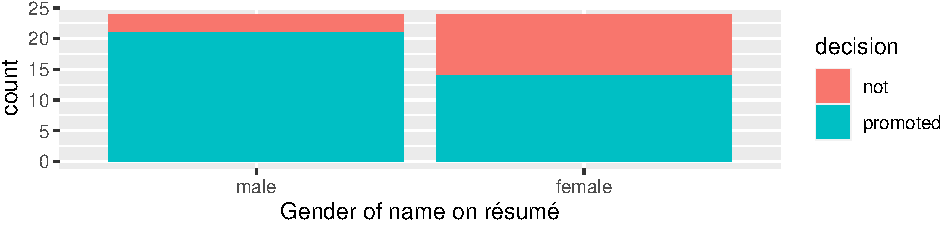
\includegraphics{tecnicas-cuantitativas_files/figure-latex/promotions-barplot-1.pdf}
\caption{\label{fig:promotions-barplot}Barplot relating gender to promotion decision.}
\end{figure}

Observe in Figure \ref{fig:promotions-barplot} that it appears that résumés with female names were much less likely to be accepted for promotion. Let's quantify these promotion rates by computing the proportion of résumés accepted for promotion for each group using the \texttt{dplyr} package for data wrangling. Note the use of the \texttt{tally()} function here which is a shortcut for \texttt{summarize(n\ =\ n())} to get counts.

\begin{Shaded}
\begin{Highlighting}[]
\NormalTok{promotions }\OperatorTok\StringTok{ }
\StringTok{  }\KeywordTok{group_by}\NormalTok{(gender, decision) }\OperatorTok\StringTok{ }
\StringTok{  }\KeywordTok{tally}\NormalTok{()}
\end{Highlighting}
\end{Shaded}

\begin{verbatim}
## # A tibble: 4 x 3
## # Groups:   gender [2]
##   gender decision     n
##   <fct>  <fct>    <int>
## 1 male   not          3
## 2 male   promoted    21
## 3 female not         10
## 4 female promoted    14
\end{verbatim}

So of the 24 résumés with male names, 21 were selected for promotion, for a proportion of 21/24 = 0.875 = 87.5\%. On the other hand, of the 24 résumés with female names, 14 were selected for promotion, for a proportion of 14/24 = 0.583 = 58.3\%. Comparing these two rates of promotion, it appears that résumés with male names were selected for promotion at a rate 0.875 - 0.583 = 0.292 = 29.2\% higher than résumés with female names. This is suggestive of an advantage for résumés with a male name on it.

The question is, however, does this provide \emph{conclusive} evidence that there is gender discrimination in promotions at banks? Could a difference in promotion rates of 29.2\% still occur by chance, even in a hypothetical world where no gender-based discrimination existed? In other words, what is the role of \emph{sampling variation} in this hypothesized world? To answer this question, we'll again rely on a computer to run \emph{simulations}.

\hypertarget{shuffling-once}{%
\subsection{Shuffling once}\label{shuffling-once}}

First, try to imagine a hypothetical universe where no gender discrimination in promotions existed. In such a hypothetical universe, the gender of an applicant would have no bearing on their chances of promotion. Bringing things back to our \texttt{promotions} data frame, the \texttt{gender} variable would thus be an irrelevant label. If these \texttt{gender} labels were irrelevant, then we could randomly reassign them by ``shuffling'' them to no consequence!

To illustrate this idea, let's narrow our focus to 6 arbitrarily chosen résumés of the 48 in Table \ref{tab:compare-six}. The \texttt{decision} column shows that 3 résumés resulted in promotion while 3 didn't. The \texttt{gender} column shows what the original gender of the résumé name was.

However, in our hypothesized universe of no gender discrimination, gender is irrelevant and thus it is of no consequence to randomly ``shuffle'' the values of \texttt{gender}. The \texttt{shuffled\_gender} column shows one such possible random shuffling. Observe in the fourth column how the number of male and female names remains the same at 3 each, but they are now listed in a different order.

\label{tab:compare-six}One example of shuffling gender variable

résumé number

decision

gender

shuffled gender

1

not

male

male

2

not

female

male

3

not

female

female

4

promoted

male

female

5

promoted

male

female

6

promoted

female

male

Again, such random shuffling of the gender label only makes sense in our hypothesized universe of no gender discrimination. How could we extend this shuffling of the gender variable to all 48 résumés by hand? One way would be by using standard deck of 52 playing cards, which we display in Figure \ref{fig:deck-of-cards}.

Since half the cards are red (diamonds and hearts) and the other half are black (spades and clubs), by removing two red cards and two black cards, we would end up with 24 red cards and 24 black cards. After shuffling these 48 cards as seen in Figure \ref{fig:shuffling}, we can flip the cards over one-by-one, assigning ``male'' for each red card and ``female'' for each black card.

We've saved one such shuffling in the \texttt{promotions\_shuffled} data frame of the \texttt{moderndive} package. If you compare the original \texttt{promotions} and the shuffled \texttt{promotions\_shuffled} data frames, you'll see that while the \texttt{decision} variable is identical, the \texttt{gender} variable has changed.

Let's repeat the same exploratory data analysis we did for the original \texttt{promotions} data on our \texttt{promotions\_shuffled} data frame. Let's create a barplot visualizing the relationship between \texttt{decision} and the new shuffled \texttt{gender} variable and compare this to the original unshuffled version in Figure \ref{fig:promotions-barplot-permuted}.

\begin{Shaded}
\begin{Highlighting}[]
\KeywordTok{ggplot}\NormalTok{(promotions_shuffled, }
       \KeywordTok{aes}\NormalTok{(}\DataTypeTok{x =}\NormalTok{ gender, }\DataTypeTok{fill =}\NormalTok{ decision)) }\OperatorTok{+}
\StringTok{  }\KeywordTok{geom_bar}\NormalTok{() }\OperatorTok{+}\StringTok{ }
\StringTok{  }\KeywordTok{labs}\NormalTok{(}\DataTypeTok{x =} \StringTok{"Gender of résumé name"}\NormalTok{)}
\end{Highlighting}
\end{Shaded}

\begin{verbatim}
## `summarise()` regrouping output by 'gender' (override with `.groups` argument)
## `summarise()` regrouping output by 'gender' (override with `.groups` argument)
\end{verbatim}

\begin{figure}
\centering
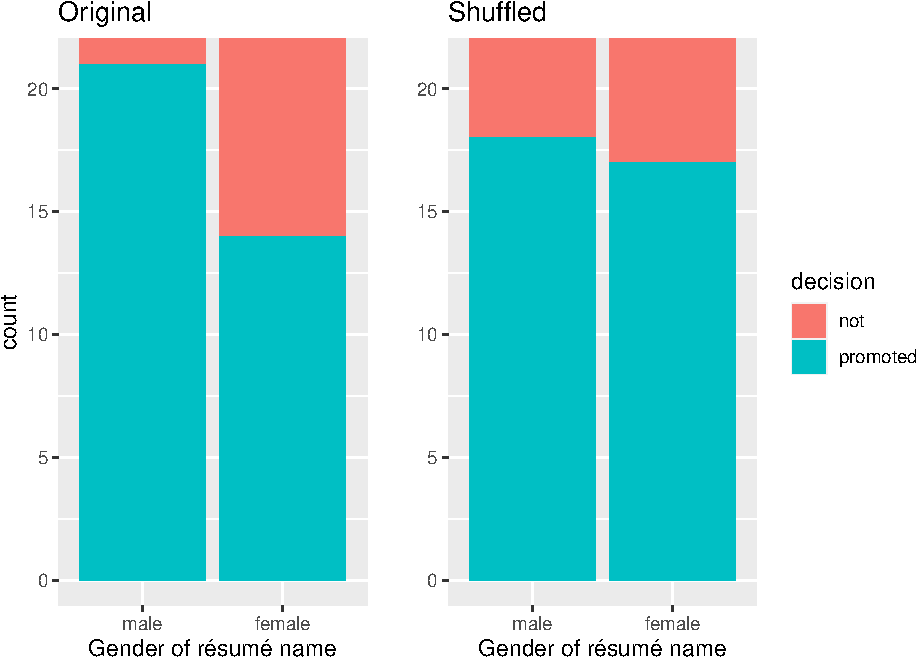
\includegraphics{tecnicas-cuantitativas_files/figure-latex/promotions-barplot-permuted-1.pdf}
\caption{\label{fig:promotions-barplot-permuted}Barplots of relationship of promotion with gender (left) and shuffled gender (right).}
\end{figure}

It appears the difference in ``male names'' versus ``female names'' promotion rates is now different. Compared to the original data in the left barplot, the new ``shuffled'' data in the right barplot has promotion rates that are much more similar.

Let's also compute the proportion of résumés accepted for promotion for each group:

\begin{Shaded}
\begin{Highlighting}[]
\NormalTok{promotions_shuffled }\OperatorTok\StringTok{ }
\StringTok{  }\KeywordTok{group_by}\NormalTok{(gender, decision) }\OperatorTok\StringTok{ }
\StringTok{  }\KeywordTok{tally}\NormalTok{() }\CommentTok{# Same as summarize(n = n())}
\end{Highlighting}
\end{Shaded}

\begin{verbatim}
## # A tibble: 4 x 3
## # Groups:   gender [2]
##   gender decision     n
##   <fct>  <fct>    <int>
## 1 male   not          6
## 2 male   promoted    18
## 3 female not          7
## 4 female promoted    17
\end{verbatim}

So in this hypothetical universe of no discrimination, \(18/24 = 0.75 = 75\%\) of ``male'' résumés were selected for promotion. On the other hand, \(17/24 = 0.708 = 70.8\%\) of ``female'' résumés were selected for promotion.

Let's next compare these two values. It appears that résumés with stereotypically male names were selected for promotion at a rate that was \(0.75 - 0.708 = 0.042 = 4.2\%\) different than résumés with stereotypically female names.

Observe how this difference in rates is not the same as the difference in rates of 0.292 = 29.2\% we originally observed. This is once again due to \emph{sampling variation}. How can we better understand the effect of this sampling variation? By repeating this shuffling several times!

\hypertarget{shuffling-16-times}{%
\subsection{Shuffling 16 times}\label{shuffling-16-times}}

We recruited 16 groups of our friends to repeat this shuffling exercise. They recorded these values in a \href{https://docs.google.com/spreadsheets/d/1Q-ENy3o5IrpJshJ7gn3hJ5A0TOWV2AZrKNHMsshQtiE/}{shared spreadsheet}; we display a snapshot of the first 10 rows and 5 columns in Figure \ref{fig:tactile-shuffling}.

For each of these 16 columns of \emph{shuffles}, we computed the difference in promotion rates, and in Figure \ref{fig:null-distribution-1} we display their distribution in a histogram. We also mark the observed difference in promotion rate that occurred in real life of 0.292 = 29.2\% with a dark line.

\begin{figure}
\centering
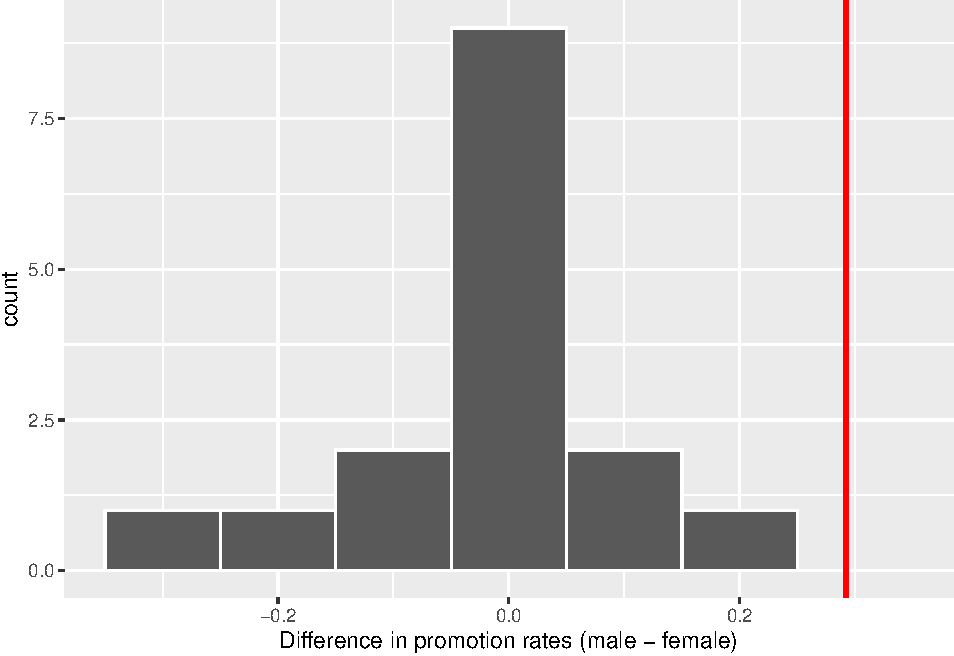
\includegraphics{tecnicas-cuantitativas_files/figure-latex/null-distribution-1-1.pdf}
\caption{\label{fig:null-distribution-1}Distribution of shuffled differences in promotions.}
\end{figure}

Before we discuss the distribution of the histogram, we emphasize the key thing to remember: this histogram represents differences in promotion rates that one would observe in our \emph{hypothesized universe} of no gender discrimination.

Observe first that the histogram is roughly centered at 0. Saying that the difference in promotion rates is 0 is equivalent to saying that both genders had the same promotion rate. In other words, the center of these 16 values is consistent with what we would expect in our hypothesized universe of no gender discrimination.

However, while the values are centered at 0, there is variation about 0. This is because even in a hypothesized universe of no gender discrimination, you will still likely observe small differences in promotion rates because of chance \emph{sampling variation}. Looking at the histogram in Figure \ref{fig:null-distribution-1}, such differences could even be as extreme as -0.292 or 0.208.

Turning our attention to what we observed in real life: the difference of 0.292 = 29.2\% is marked with a vertical dark line. Ask yourself: in a hypothesized world of no gender discrimination, how likely would it be that we observe this difference? While opinions here may differ, in our opinion not often! Now ask yourself: what do these results say about our hypothesized universe of no gender discrimination?

\hypertarget{ht-what-did-we-just-do}{%
\subsection{What did we just do?}\label{ht-what-did-we-just-do}}

What we just demonstrated in this activity is the statistical procedure known as \emph{hypothesis testing} using a \emph{permutation test}. The term ``permutation'' \index{permutation} is the mathematical term for ``shuffling'': taking a series of values and reordering them randomly, as you did with the playing cards.

In fact, permutations are another form of \emph{resampling}, like the bootstrap method you performed in Chapter \ref{confidence-intervals}. While the bootstrap method involves resampling \emph{with} replacement, permutation methods involve resampling \emph{without} replacement.

Think of our exercise involving the slips of paper representing pennies and the hat in Section \ref{resampling-tactile}: after sampling a penny, you put it back in the hat. Now think of our deck of cards. After drawing a card, you laid it out in front of you, recorded the color, and then you \emph{did not} put it back in the deck.

In our previous example, we tested the validity of the hypothesized universe of no gender discrimination. The evidence contained in our observed sample of 48 résumés was somewhat inconsistent with our hypothesized universe. Thus, we would be inclined to \emph{reject} this hypothesized universe and declare that the evidence suggests there is gender discrimination.

Recall our case study on whether yawning is contagious from Section \ref{case-study-two-prop-ci}. The previous example involves inference about an unknown difference of population proportions as well. This time, it will be \(p_{m} - p_{f}\), where \(p_{m}\) is the population proportion of résumés with male names being recommended for promotion and \(p_{f}\) is the equivalent for résumés with female names. Recall that this is one of the scenarios for inference we've seen so far in Table \ref{tab:table-diff-prop}.

\label{tab:table-diff-prop}Scenarios of sampling for inference

Scenario

Population parameter

Notation

Point estimate

Symbol(s)

1

Population proportion

\(p\)

Sample proportion

\(\widehat{p}\)

2

Population mean

\(\mu\)

Sample mean

\(\overline{x}\) or \(\widehat{\mu}\)

3

Difference in population proportions

\(p_1 - p_2\)

Difference in sample proportions

\(\widehat{p}_1 - \widehat{p}_2\)

So, based on our sample of \(n_m\) = 24 ``male'' applicants and \(n_w\) = 24 ``female'' applicants, the \emph{point estimate} for \(p_{m} - p_{f}\) is the \emph{difference in sample proportions} \(\widehat{p}_{m} -\widehat{p}_{f}\) = 0.875 - 0.583 = 0.292 = 29.2\%. This difference in favor of ``male'' résumés of 0.292 is greater than 0, suggesting discrimination in favor of men.

However, the question we asked ourselves was ``is this difference meaningfully greater than 0?''. In other words, is that difference indicative of true discrimination, or can we just attribute it to \emph{sampling variation}? Hypothesis testing allows us to make such distinctions.

\hypertarget{understanding-ht}{%
\section{Understanding hypothesis tests}\label{understanding-ht}}

Much like the terminology, notation, and definitions relating to sampling you saw in Section \ref{sampling-framework}, there are a lot of terminology, notation, and definitions related to hypothesis testing as well. Learning these may seem like a very daunting task at first. However, with practice, practice, and more practice, anyone can master them.

First, a \textbf{hypothesis} \index{hypothesis testing!hypothesis} is a statement about the value of an unknown population parameter. In our résumé activity, our population parameter of interest is the difference in population proportions \(p_{m} - p_{f}\). Hypothesis tests can involve any of the population parameters in Table \ref{tab:table-ch8} of the five inference scenarios we'll cover in this book and also more advanced types we won't cover here.

Second, a \textbf{hypothesis test} \index{hypothesis testing} consists of a test between two competing hypotheses: (1) a \textbf{null hypothesis} \(H_0\) (pronounced ``H-naught'') versus (2) an \textbf{alternative hypothesis} \(H_A\) (also denoted \(H_1\)).

Generally the null hypothesis \index{hypothesis testing!null hypothesis} is a claim that there is ``no effect'' or ``no difference of interest.'' In many cases, the null hypothesis represents the status quo or a situation that nothing interesting is happening. Furthermore, generally the alternative hypothesis \index{hypothesis testing!alternative hypothesis} is the claim the experimenter or researcher wants to establish or find evidence to support. It is viewed as a ``challenger'' hypothesis to the null hypothesis \(H_0\). In our résumé activity, an appropriate hypothesis test would be:

\[
\begin{aligned}
H_0 &: \text{men and women are promoted at the same rate}\\
\text{vs } H_A &: \text{men are promoted at a higher rate than women}
\end{aligned}
\]

Note some of the choices we have made. First, we set the null hypothesis \(H_0\) to be that there is no difference in promotion rate and the ``challenger'' alternative hypothesis \(H_A\) to be that there is a difference. While it would not be wrong in principle to reverse the two, it is a convention in statistical inference that the null hypothesis is set to reflect a ``null'' situation where ``nothing is going on.'' As we discussed earlier, in this case, \(H_0\) corresponds to there being no difference in promotion rates. Furthermore, we set \(H_A\) to be that men are promoted at a \emph{higher} rate, a subjective choice reflecting a prior suspicion we have that this is the case. We call such alternative hypotheses \index{hypothesis testing!one-sided alternative} \emph{one-sided alternatives}. If someone else however does not share such suspicions and only wants to investigate that there is a difference, whether higher or lower, they would set what is known as a \index{hypothesis testing!two-sided alternative} \emph{two-sided alternative}.

We can re-express the formulation of our hypothesis test using the mathematical notation for our population parameter of interest, the difference in population proportions \(p_{m} - p_{f}\):

\[
\begin{aligned}
H_0 &: p_{m} - p_{f} = 0\\
\text{vs } H_A&: p_{m} - p_{f} > 0
\end{aligned}
\]

Observe how the alternative hypothesis \(H_A\) is one-sided with \(p_{m} - p_{f} > 0\). Had we opted for a two-sided alternative, we would have set \(p_{m} - p_{f} \neq 0\). To keep things simple for now, we'll stick with the simpler one-sided alternative. We'll present an example of a two-sided alternative in Section \ref{ht-case-study}.

Third, a \textbf{test statistic} \index{hypothesis testing!test statistic} is a \emph{point estimate/sample statistic} formula used for hypothesis testing. Note that a sample statistic is merely a summary statistic based on a sample of observations. Recall we saw in Section \ref{summarize} that a summary statistic takes in many values and returns only one. Here, the samples would be the \(n_m\) = 24 résumés with male names and the \(n_f\) = 24 résumés with female names. Hence, the point estimate of interest is the difference in sample proportions \(\widehat{p}_{m} - \widehat{p}_{f}\).

Fourth, the \textbf{observed test statistic} \index{hypothesis testing!observed test statistic} is the value of the test statistic that we observed in real life. In our case, we computed this value using the data saved in the \texttt{promotions} data frame. It was the observed difference of \(\widehat{p}_{m} -\widehat{p}_{f} = 0.875 - 0.583 = 0.292 = 29.2\%\) in favor of résumés with male names.

Fifth, the \textbf{null distribution} \index{hypothesis testing!null distribution} is the sampling distribution of the test statistic \emph{assuming the null hypothesis \(H_0\) is true}. Ooof! That's a long one! Let's unpack it slowly. The key to understanding the null distribution is that the null hypothesis \(H_0\) is \emph{assumed} to be true. We're not saying that \(H_0\) is true at this point, we're only assuming it to be true for hypothesis testing purposes. In our case, this corresponds to our hypothesized universe of no gender discrimination in promotion rates. Assuming the null hypothesis \(H_0\), also stated as ``Under \(H_0\),'' how does the test statistic vary due to sampling variation? In our case, how will the difference in sample proportions \(\widehat{p}_{m} - \widehat{p}_{f}\) vary due to sampling under \(H_0\)? Recall from Subsection \ref{sampling-definitions} that distributions displaying how point estimates vary due to sampling variation are called \emph{sampling distributions}. The only additional thing to keep in mind about null distributions is that they are sampling distributions \emph{assuming the null hypothesis \(H_0\) is true}.

In our case, we previously visualized a null distribution in Figure \ref{fig:null-distribution-1}, which we re-display in Figure \ref{fig:null-distribution-2} using our new notation and terminology. It is the distribution of the 16 differences in sample proportions our friends computed \emph{assuming} a hypothetical universe of no gender discrimination. We also mark the value of the observed test statistic of 0.292 with a vertical line.

\begin{figure}
\centering
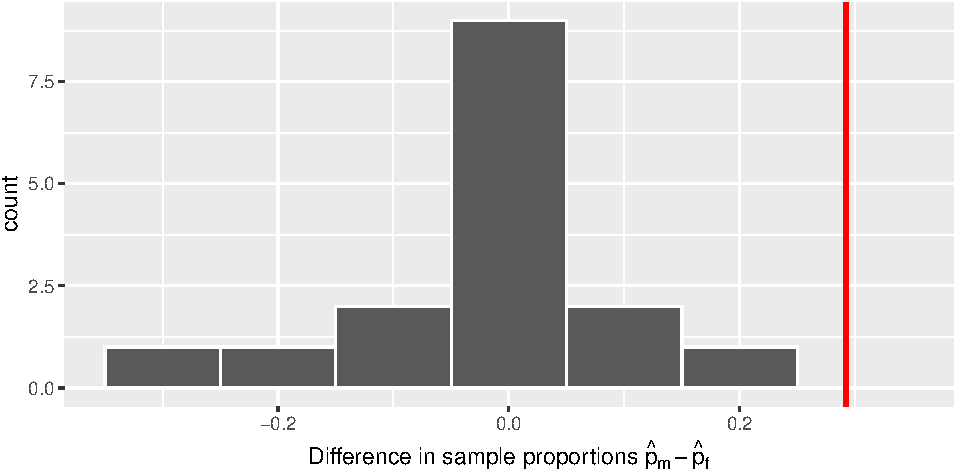
\includegraphics{tecnicas-cuantitativas_files/figure-latex/null-distribution-2-1.pdf}
\caption{\label{fig:null-distribution-2}Null distribution and observed test statistic.}
\end{figure}

Sixth, the \textbf{\(p\)-value} \index{hypothesis testing!p-value} is the probability of obtaining a test statistic just as extreme or more extreme than the observed test statistic \emph{assuming the null hypothesis \(H_0\) is true}. Double ooof! Let's unpack this slowly as well. You can think of the \(p\)-value as a quantification of ``surprise'': assuming \(H_0\) is true, how surprised are we with what we observed? Or in our case, in our hypothesized universe of no gender discrimination, how surprised are we that we observed a difference in promotion rates of 0.292 from our collected samples assuming \(H_0\) is true? Very surprised? Somewhat surprised?

The \(p\)-value quantifies this probability, or in the case of our 16 differences in sample proportions in Figure \ref{fig:null-distribution-2}, what proportion had a more ``extreme'' result? Here, extreme is defined in terms of the alternative hypothesis \(H_A\) that ``male'' applicants are promoted at a higher rate than ``female'' applicants. In other words, how often was the discrimination in favor of men \emph{even more} pronounced than \(0.875 - 0.583 = 0.292 = 29.2\%\)?

In this case, 0 times out of 16, we obtained a difference in proportion greater than or equal to the observed difference of 0.292 = 29.2\%. A very rare (in fact, not occurring) outcome! Given the rarity of such a pronounced difference in promotion rates in our hypothesized universe of no gender discrimination, we're inclined to \emph{reject} \index{hypothesis testing!reject the null hypothesis} our hypothesized universe. Instead, we favor the hypothesis stating there is discrimination in favor of the ``male'' applicants. In other words, we reject \(H_0\) in favor of \(H_A\).

Seventh and lastly, in many hypothesis testing procedures, it is commonly recommended to set the \textbf{significance level} \index{hypothesis testing!significance level} of the test beforehand. It is denoted by the Greek letter \(\alpha\) (pronounced ``alpha''). This value acts as a cutoff on the \(p\)-value, where if the \(p\)-value falls below \(\alpha\), we would ``reject the null hypothesis \(H_0\).''

Alternatively, if the \(p\)-value does not fall below \(\alpha\), we would ``fail to reject \(H_0\).'' Note the latter statement is not quite the same as saying we ``accept \(H_0\).'' This distinction is rather subtle and not immediately obvious. So we'll revisit it later in Section \ref{ht-interpretation}.

While different fields tend to use different values of \(\alpha\), some commonly used values for \(\alpha\) are 0.1, 0.01, and 0.05; with 0.05 being the choice people often make without putting much thought into it. We'll talk more about \(\alpha\) significance levels in Section \ref{ht-interpretation}, but first let's fully conduct the hypothesis test corresponding to our promotions activity using the \texttt{infer} package.

\hypertarget{ht-infer}{%
\section{Conducting hypothesis tests}\label{ht-infer}}

In Section \ref{bootstrap-process}, we showed you how to construct confidence intervals. We first illustrated how to do this using \texttt{dplyr} data wrangling verbs and the \texttt{rep\_sample\_n()} function from Subsection \ref{shovel-1000-times} which we used as a virtual shovel. In particular, we constructed confidence intervals by resampling with replacement by setting the \texttt{replace\ =\ TRUE} argument to the \texttt{rep\_sample\_n()} function.

We then showed you how to perform the same task using the \texttt{infer} package workflow. While both workflows resulted in the same bootstrap distribution from which we can construct confidence intervals, the \texttt{infer} package workflow emphasizes each of the steps in the overall process in Figure \ref{fig:infer-ci}. It does so using function names that are intuitively named with verbs:

\begin{enumerate}
\def\labelenumi{\arabic{enumi}.}
\tightlist
\item
  \texttt{specify()} the variables of interest in your data frame.
\item
  \texttt{generate()} replicates of bootstrap resamples with replacement.
\item
  \texttt{calculate()} the summary statistic of interest.
\item
  \texttt{visualize()} the resulting bootstrap distribution and confidence interval.
\end{enumerate}

In this section, we'll now show you how to seamlessly modify the previously seen \texttt{infer} code for constructing confidence intervals to conduct hypothesis tests. You'll notice that the basic outline of the workflow is almost identical, except for an additional \texttt{hypothesize()} step between the \texttt{specify()} and \texttt{generate()} steps, as can be seen in Figure \ref{fig:inferht}.

Furthermore, we'll use a pre-specified significance level \(\alpha\) = 0.05 for this hypothesis test. Let's leave discussion on the choice of this \(\alpha\) value until later on in Section \ref{ht-interpretation}.

\hypertarget{infer-workflow-ht}{%
\subsection{\texorpdfstring{\texttt{infer} package workflow}{infer package workflow}}\label{infer-workflow-ht}}

\hypertarget{specify-variables}{%
\subsubsection*{\texorpdfstring{1. \texttt{specify} variables}{1. specify variables}}\label{specify-variables}}
\addcontentsline{toc}{subsubsection}{1. \texttt{specify} variables}

Recall that we use the \texttt{specify()} \index{infer!specify()} verb to specify the response variable and, if needed, any explanatory variables for our study. In this case, since we are interested in any potential effects of gender on promotion decisions, we set \texttt{decision} as the response variable and \texttt{gender} as the explanatory variable. We do so using \texttt{formula\ =\ response\ \textasciitilde{}\ explanatory} where \texttt{response} is the name of the response variable in the data frame and \texttt{explanatory} is the name of the explanatory variable. So in our case it is \texttt{decision\ \textasciitilde{}\ gender}.

Furthermore, since we are interested in the proportion of résumés \texttt{"promoted"}, and not the proportion of résumés \texttt{not} promoted, we set the argument \texttt{success} to \texttt{"promoted"}.

\begin{Shaded}
\begin{Highlighting}[]
\NormalTok{promotions }\OperatorTok\StringTok{ }
\StringTok{  }\KeywordTok{specify}\NormalTok{(}\DataTypeTok{formula =}\NormalTok{ decision }\OperatorTok{~}\StringTok{ }\NormalTok{gender, }\DataTypeTok{success =} \StringTok{"promoted"}\NormalTok{) }
\end{Highlighting}
\end{Shaded}

\begin{verbatim}
## Response: decision (factor)
## Explanatory: gender (factor)
## # A tibble: 48 x 2
##    decision gender
##    <fct>    <fct> 
##  1 promoted male  
##  2 promoted male  
##  3 promoted male  
##  4 promoted male  
##  5 promoted male  
##  6 promoted male  
##  7 promoted male  
##  8 promoted male  
##  9 promoted male  
## 10 promoted male  
## # ... with 38 more rows
\end{verbatim}

Again, notice how the \texttt{promotions} data itself doesn't change, but the \texttt{Response:\ decision\ (factor)} and \texttt{Explanatory:\ gender\ (factor)} \emph{meta-data} do. This is similar to how the \texttt{group\_by()} verb from \texttt{dplyr} doesn't change the data, but only adds ``grouping'' meta-data, as we saw in Section \ref{groupby}.

\hypertarget{hypothesize-the-null}{%
\subsubsection*{\texorpdfstring{2. \texttt{hypothesize} the null}{2. hypothesize the null}}\label{hypothesize-the-null}}
\addcontentsline{toc}{subsubsection}{2. \texttt{hypothesize} the null}

In order to conduct hypothesis tests using the \texttt{infer} workflow, we need a new step not present for confidence intervals: \index{infer!hypothesize()} \texttt{hypothesize()}. Recall from Section \ref{understanding-ht} that our hypothesis test was

\[
\begin{aligned}
H_0 &: p_{m} - p_{f} = 0\\
\text{vs. } H_A&: p_{m} - p_{f} > 0
\end{aligned}
\]

In other words, the null hypothesis \(H_0\) corresponding to our ``hypothesized universe'' stated that there was no difference in gender-based discrimination rates. We set this null hypothesis \(H_0\) in our \texttt{infer} workflow using the \texttt{null} argument of the \texttt{hypothesize()} function to either:

\begin{itemize}
\tightlist
\item
  \texttt{"point"} for hypotheses involving a single sample or
\item
  \texttt{"independence"} for hypotheses involving two samples.
\end{itemize}

In our case, since we have two samples (the résumés with ``male'' and ``female'' names), we set \texttt{null\ =\ "independence"}.

\begin{Shaded}
\begin{Highlighting}[]
\NormalTok{promotions }\OperatorTok\StringTok{ }
\StringTok{  }\KeywordTok{specify}\NormalTok{(}\DataTypeTok{formula =}\NormalTok{ decision }\OperatorTok{~}\StringTok{ }\NormalTok{gender, }\DataTypeTok{success =} \StringTok{"promoted"}\NormalTok{) }\OperatorTok\StringTok{ }
\StringTok{  }\KeywordTok{hypothesize}\NormalTok{(}\DataTypeTok{null =} \StringTok{"independence"}\NormalTok{)}
\end{Highlighting}
\end{Shaded}

\begin{verbatim}
## Response: decision (factor)
## Explanatory: gender (factor)
## Null Hypothesis: independence
## # A tibble: 48 x 2
##    decision gender
##    <fct>    <fct> 
##  1 promoted male  
##  2 promoted male  
##  3 promoted male  
##  4 promoted male  
##  5 promoted male  
##  6 promoted male  
##  7 promoted male  
##  8 promoted male  
##  9 promoted male  
## 10 promoted male  
## # ... with 38 more rows
\end{verbatim}

Again, the data has not changed yet. This will occur at the upcoming \texttt{generate()} step; we're merely setting meta-data for now.

Where do the terms \texttt{"point"} and \texttt{"independence"} come from? These are two technical statistical terms. The term ``point'' relates from the fact that for a single group of observations, you will test the value of a single point. Going back to the pennies example from Chapter \ref{confidence-intervals}, say we wanted to test if the mean year of all US pennies was equal to 1993 or not. We would be testing the value of a ``point'' \(\mu\), the mean year of \emph{all} US pennies, as follows

\[
\begin{aligned}
H_0 &: \mu = 1993\\
\text{vs } H_A&: \mu \neq 1993
\end{aligned}
\]

The term ``independence'' relates to the fact that for two groups of observations, you are testing whether or not the response variable is \emph{independent} of the explanatory variable that assigns the groups. In our case, we are testing whether the \texttt{decision} response variable is ``independent'' of the explanatory variable \texttt{gender} that assigns each résumé to either of the two groups.

\hypertarget{generate-replicates}{%
\subsubsection*{\texorpdfstring{3. \texttt{generate} replicates}{3. generate replicates}}\label{generate-replicates}}
\addcontentsline{toc}{subsubsection}{3. \texttt{generate} replicates}

After we \texttt{hypothesize()} the null hypothesis, we \texttt{generate()} replicates of ``shuffled'' datasets assuming the null hypothesis is true. We do this by repeating the shuffling exercise you performed in Section \ref{ht-activity} several times. Instead of merely doing it 16 times as our groups of friends did, let's use the computer to repeat this 1000 times by setting \texttt{reps\ =\ 1000} in the \texttt{generate()} \index{infer!generate()} function. However, unlike for confidence intervals where we generated replicates using \texttt{type\ =\ "bootstrap"} resampling with replacement, we'll now perform shuffles/permutations by setting \texttt{type\ =\ "permute"}. Recall that shuffles/permutations are a kind of resampling, but unlike the bootstrap method, they involve resampling \emph{without} replacement.

\begin{Shaded}
\begin{Highlighting}[]
\NormalTok{promotions_generate <-}\StringTok{ }\NormalTok{promotions }\OperatorTok\StringTok{ }
\StringTok{  }\KeywordTok{specify}\NormalTok{(}\DataTypeTok{formula =}\NormalTok{ decision }\OperatorTok{~}\StringTok{ }\NormalTok{gender, }\DataTypeTok{success =} \StringTok{"promoted"}\NormalTok{) }\OperatorTok\StringTok{ }
\StringTok{  }\KeywordTok{hypothesize}\NormalTok{(}\DataTypeTok{null =} \StringTok{"independence"}\NormalTok{) }\OperatorTok\StringTok{ }
\StringTok{  }\KeywordTok{generate}\NormalTok{(}\DataTypeTok{reps =} \DecValTok{1000}\NormalTok{, }\DataTypeTok{type =} \StringTok{"permute"}\NormalTok{)}
\KeywordTok{nrow}\NormalTok{(promotions_generate)}
\end{Highlighting}
\end{Shaded}

\begin{verbatim}
## [1] 48000
\end{verbatim}

Observe that the resulting data frame has 48,000 rows. This is because we performed shuffles/permutations for each of the 48 rows 1000 times and \(48,000 = 1000 \cdot 48\). If you explore the \texttt{promotions\_generate} data frame with \texttt{View()}, you'll notice that the variable \texttt{replicate} indicates which resample each row belongs to. So it has the value \texttt{1} 48 times, the value \texttt{2} 48 times, all the way through to the value \texttt{1000} 48 times.

\hypertarget{calculate-summary-statistics}{%
\subsubsection*{\texorpdfstring{4. \texttt{calculate} summary statistics}{4. calculate summary statistics}}\label{calculate-summary-statistics}}
\addcontentsline{toc}{subsubsection}{4. \texttt{calculate} summary statistics}

Now that we have generated 1000 replicates of ``shuffles'' assuming the null hypothesis is true, let's \texttt{calculate()} \index{infer!calculate()} the appropriate summary statistic for each of our 1000 shuffles. From Section \ref{understanding-ht}, point estimates related to hypothesis testing have a specific name: \emph{test statistics}. Since the unknown population parameter of interest is the difference in population proportions \(p_{m} - p_{f}\), the test statistic here is the difference in sample proportions \(\widehat{p}_{m} - \widehat{p}_{f}\).

For each of our 1000 shuffles, we can calculate this test statistic by setting \texttt{stat\ =\ "diff\ in\ props"}. Furthermore, since we are interested in \(\widehat{p}_{m} - \widehat{p}_{f}\) we set \texttt{order\ =\ c("male",\ "female")}. As we stated earlier, the order of the subtraction does not matter, so long as you stay consistent throughout your analysis and tailor your interpretations accordingly.

Let's save the result in a data frame called \texttt{null\_distribution}:

\begin{Shaded}
\begin{Highlighting}[]
\NormalTok{null_distribution <-}\StringTok{ }\NormalTok{promotions }\OperatorTok\StringTok{ }
\StringTok{  }\KeywordTok{specify}\NormalTok{(}\DataTypeTok{formula =}\NormalTok{ decision }\OperatorTok{~}\StringTok{ }\NormalTok{gender, }\DataTypeTok{success =} \StringTok{"promoted"}\NormalTok{) }\OperatorTok\StringTok{ }
\StringTok{  }\KeywordTok{hypothesize}\NormalTok{(}\DataTypeTok{null =} \StringTok{"independence"}\NormalTok{) }\OperatorTok\StringTok{ }
\StringTok{  }\KeywordTok{generate}\NormalTok{(}\DataTypeTok{reps =} \DecValTok{1000}\NormalTok{, }\DataTypeTok{type =} \StringTok{"permute"}\NormalTok{) }\OperatorTok\StringTok{ }
\StringTok{  }\KeywordTok{calculate}\NormalTok{(}\DataTypeTok{stat =} \StringTok{"diff in props"}\NormalTok{, }\DataTypeTok{order =} \KeywordTok{c}\NormalTok{(}\StringTok{"male"}\NormalTok{, }\StringTok{"female"}\NormalTok{))}
\NormalTok{null_distribution}
\end{Highlighting}
\end{Shaded}

\begin{verbatim}
## # A tibble: 1,000 x 2
##    replicate    stat
##        <int>   <dbl>
##  1         1 -0.0417
##  2         2 -0.125 
##  3         3 -0.125 
##  4         4 -0.0417
##  5         5 -0.0417
##  6         6 -0.125 
##  7         7 -0.125 
##  8         8 -0.125 
##  9         9 -0.0417
## 10        10 -0.0417
## # ... with 990 more rows
\end{verbatim}

Observe that we have 1000 values of \texttt{stat}, each representing one instance of \(\widehat{p}_{m} - \widehat{p}_{f}\) in a hypothesized world of no gender discrimination. Observe as well that we chose the name of this data frame carefully: \texttt{null\_distribution}. Recall once again from Section \ref{understanding-ht} that sampling distributions when the null hypothesis \(H_0\) is assumed to be true have a special name: the \emph{null distribution}.

What was the \emph{observed} difference in promotion rates? In other words, what was the \emph{observed test statistic} \(\widehat{p}_{m} - \widehat{p}_{f}\)? Recall from Section \ref{ht-activity} that we computed this observed difference by hand to be 0.875 - 0.583 = 0.292 = 29.2\%. We can also compute this value using the previous \texttt{infer} code but with the \texttt{hypothesize()} and \texttt{generate()} steps removed. Let's save this in \texttt{obs\_diff\_prop}:

\begin{Shaded}
\begin{Highlighting}[]
\NormalTok{obs_diff_prop <-}\StringTok{ }\NormalTok{promotions }\OperatorTok\StringTok{ }
\StringTok{  }\KeywordTok{specify}\NormalTok{(decision }\OperatorTok{~}\StringTok{ }\NormalTok{gender, }\DataTypeTok{success =} \StringTok{"promoted"}\NormalTok{) }\OperatorTok\StringTok{ }
\StringTok{  }\KeywordTok{calculate}\NormalTok{(}\DataTypeTok{stat =} \StringTok{"diff in props"}\NormalTok{, }\DataTypeTok{order =} \KeywordTok{c}\NormalTok{(}\StringTok{"male"}\NormalTok{, }\StringTok{"female"}\NormalTok{))}
\NormalTok{obs_diff_prop}
\end{Highlighting}
\end{Shaded}

\begin{verbatim}
## # A tibble: 1 x 1
##    stat
##   <dbl>
## 1 0.292
\end{verbatim}

\hypertarget{visualize-the-p-value}{%
\subsubsection*{\texorpdfstring{5. \texttt{visualize} the p-value}{5. visualize the p-value}}\label{visualize-the-p-value}}
\addcontentsline{toc}{subsubsection}{5. \texttt{visualize} the p-value}

The final step is to measure how surprised we are by a promotion difference of 29.2\% in a hypothesized universe of no gender discrimination. If the observed difference of 0.292 is highly unlikely, then we would be inclined to reject the validity of our hypothesized universe.

We start by visualizing the \emph{null distribution} of our 1000 values of \(\widehat{p}_{m} - \widehat{p}_{f}\) using \texttt{visualize()} \index{infer!visualize()} in Figure \ref{fig:null-distribution-infer}. Recall that these are values of the difference in promotion rates assuming \(H_0\) is true. This corresponds to being in our hypothesized universe of no gender discrimination.

\begin{Shaded}
\begin{Highlighting}[]
\KeywordTok{visualize}\NormalTok{(null_distribution, }\DataTypeTok{bins =} \DecValTok{10}\NormalTok{)}
\end{Highlighting}
\end{Shaded}

\begin{figure}
\centering
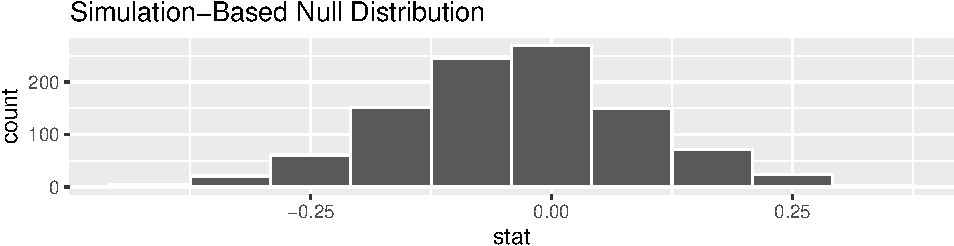
\includegraphics{tecnicas-cuantitativas_files/figure-latex/null-distribution-infer-1.pdf}
\caption{\label{fig:null-distribution-infer}Null distribution.}
\end{figure}

Let's now add what happened in real life to Figure \ref{fig:null-distribution-infer}, the observed difference in promotion rates of 0.875 - 0.583 = 0.292 = 29.2\%. However, instead of merely adding a vertical line using \texttt{geom\_vline()}, let's use the \index{infer!shade\_p\_value()} \texttt{shade\_p\_value()} function with \texttt{obs\_stat} set to the observed test statistic value we saved in \texttt{obs\_diff\_prop}.

Furthermore, we'll set the \texttt{direction\ =\ "right"} reflecting our alternative hypothesis \(H_A: p_{m} - p_{f} > 0\). Recall our alternative hypothesis \(H_A\) is that \(p_{m} - p_{f} > 0\), stating that there is a difference in promotion rates in favor of résumés with male names. ``More extreme'' here corresponds to differences that are ``bigger'' or ``more positive'' or ``more to the right.'' Hence we set the \texttt{direction} argument of \texttt{shade\_p\_value()} to be \texttt{"right"}.

On the other hand, had our alternative hypothesis \(H_A\) been the other possible one-sided alternative \(p_{m} - p_{f} < 0\), suggesting discrimination in favor of résumés with female names, we would've set \texttt{direction\ =\ "left"}. Had our alternative hypothesis \(H_A\) been two-sided \(p_{m} - p_{f} \neq 0\), suggesting discrimination in either direction, we would've set \texttt{direction\ =\ "both"}.

\begin{Shaded}
\begin{Highlighting}[]
\KeywordTok{visualize}\NormalTok{(null_distribution, }\DataTypeTok{bins =} \DecValTok{10}\NormalTok{) }\OperatorTok{+}\StringTok{ }
\StringTok{  }\KeywordTok{shade_p_value}\NormalTok{(}\DataTypeTok{obs_stat =}\NormalTok{ obs_diff_prop, }\DataTypeTok{direction =} \StringTok{"right"}\NormalTok{)}
\end{Highlighting}
\end{Shaded}

\begin{figure}
\centering
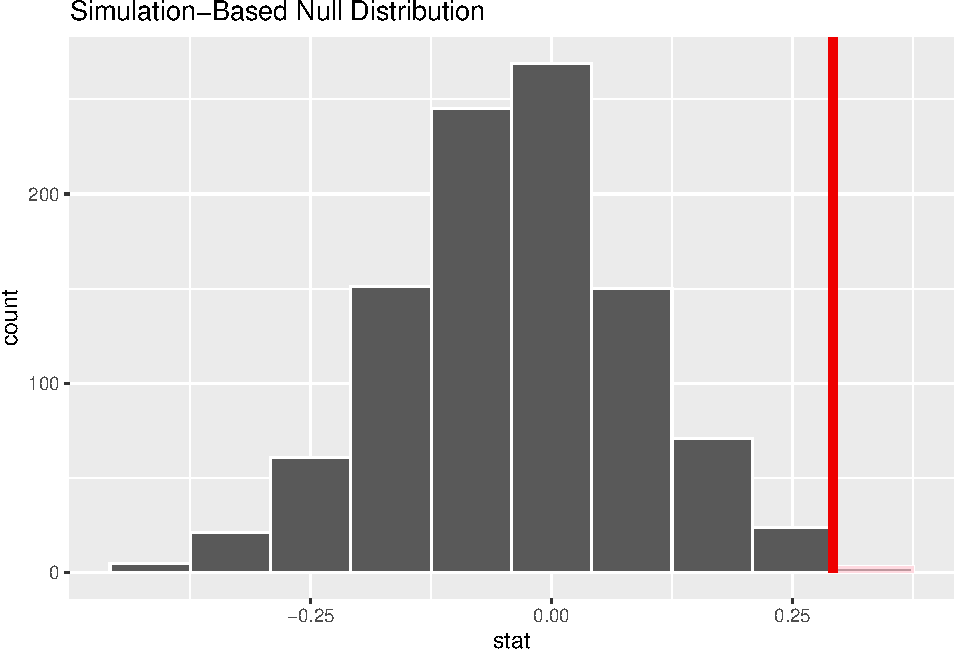
\includegraphics{tecnicas-cuantitativas_files/figure-latex/null-distribution-infer-2-1.pdf}
\caption{\label{fig:null-distribution-infer-2}Shaded histogram to show \(p\)-value.}
\end{figure}

In the resulting Figure \ref{fig:null-distribution-infer-2}, the solid dark line marks 0.292 = 29.2\%. However, what does the shaded-region correspond to? This is the \emph{\(p\)-value}. Recall the definition of the \(p\)-value from Section \ref{understanding-ht}:

\begin{quote}
A \(p\)-value is the probability of obtaining a test statistic just as or more extreme than the observed test statistic \emph{assuming the null hypothesis \(H_0\) is true}.
So judging by the shaded region in Figure \ref{fig:null-distribution-infer-2}, it seems we would somewhat rarely observe differences in promotion rates of 0.292 = 29.2\% or more in a hypothesized universe of no gender discrimination. In other words, the \(p\)-value is somewhat small. Hence, we would be inclined to reject this hypothesized universe, or using statistical language we would ``reject \(H_0\).''
\end{quote}

What fraction of the null distribution is shaded? In other words, what is the exact value of the \(p\)-value? We can compute it using the \texttt{get\_p\_value()} \index{infer!get\_p\_value()} function with the same arguments as the previous \texttt{shade\_p\_value()} code:

\begin{Shaded}
\begin{Highlighting}[]
\NormalTok{null_distribution }\OperatorTok\StringTok{ }
\StringTok{  }\KeywordTok{get_p_value}\NormalTok{(}\DataTypeTok{obs_stat =}\NormalTok{ obs_diff_prop, }\DataTypeTok{direction =} \StringTok{"right"}\NormalTok{)}
\end{Highlighting}
\end{Shaded}

\begin{verbatim}
## # A tibble: 1 x 1
##   p_value
##     <dbl>
## 1   0.027
\end{verbatim}

Keeping the definition of a \(p\)-value in mind, the probability of observing a difference in promotion rates as large as 0.292 = 29.2\% due to sampling variation alone in the null distribution is 0.027 = 2.7\%. Since this \(p\)-value is smaller than our pre-specified significance level \(\alpha\) = 0.05, we reject the null hypothesis \(H_0: p_{m} - p_{f} = 0\). In other words, this \(p\)-value is sufficiently small to reject our hypothesized universe of no gender discrimination. We instead have enough evidence to change our mind in favor of gender discrimination being a likely culprit here. Observe that whether we reject the null hypothesis \(H_0\) or not depends in large part on our choice of significance level \(\alpha\). We'll discuss this more in Subsection \ref{choosing-alpha}.

\hypertarget{comparing-infer-workflows}{%
\subsection{Comparison with confidence intervals}\label{comparing-infer-workflows}}

One of the great things about the \texttt{infer} package is that we can jump seamlessly between conducting hypothesis tests and constructing confidence intervals with minimal changes! Recall the code from the previous section that creates the null distribution, which in turn is needed to compute the \(p\)-value:

\begin{Shaded}
\begin{Highlighting}[]
\NormalTok{null_distribution <-}\StringTok{ }\NormalTok{promotions }\OperatorTok\StringTok{ }
\StringTok{  }\KeywordTok{specify}\NormalTok{(}\DataTypeTok{formula =}\NormalTok{ decision }\OperatorTok{~}\StringTok{ }\NormalTok{gender, }\DataTypeTok{success =} \StringTok{"promoted"}\NormalTok{) }\OperatorTok\StringTok{ }
\StringTok{  }\KeywordTok{hypothesize}\NormalTok{(}\DataTypeTok{null =} \StringTok{"independence"}\NormalTok{) }\OperatorTok\StringTok{ }
\StringTok{  }\KeywordTok{generate}\NormalTok{(}\DataTypeTok{reps =} \DecValTok{1000}\NormalTok{, }\DataTypeTok{type =} \StringTok{"permute"}\NormalTok{) }\OperatorTok\StringTok{ }
\StringTok{  }\KeywordTok{calculate}\NormalTok{(}\DataTypeTok{stat =} \StringTok{"diff in props"}\NormalTok{, }\DataTypeTok{order =} \KeywordTok{c}\NormalTok{(}\StringTok{"male"}\NormalTok{, }\StringTok{"female"}\NormalTok{))}
\end{Highlighting}
\end{Shaded}

To create the corresponding bootstrap distribution needed to construct a 95\% confidence interval for \(p_{m} - p_{f}\), we only need to make two changes. \index{infer!switching between tests and confidence intervals} First, we remove the \texttt{hypothesize()} step since we are no longer assuming a null hypothesis \(H_0\) is true. We can do this by deleting or commenting out the \texttt{hypothesize()} line of code. Second, we switch the \texttt{type} of resampling in the \texttt{generate()} step to be \texttt{"bootstrap"} instead of \texttt{"permute"}.

\begin{Shaded}
\begin{Highlighting}[]
\NormalTok{bootstrap_distribution <-}\StringTok{ }\NormalTok{promotions }\OperatorTok\StringTok{ }
\StringTok{  }\KeywordTok{specify}\NormalTok{(}\DataTypeTok{formula =}\NormalTok{ decision }\OperatorTok{~}\StringTok{ }\NormalTok{gender, }\DataTypeTok{success =} \StringTok{"promoted"}\NormalTok{) }\OperatorTok\StringTok{ }
\StringTok{  }\CommentTok{# Change 1 - Remove hypothesize():}
\StringTok{  }\CommentTok{# hypothesize(null = "independence") %>% }
\StringTok{  }\CommentTok{# Change 2 - Switch type from "permute" to "bootstrap":}
\StringTok{  }\KeywordTok{generate}\NormalTok{(}\DataTypeTok{reps =} \DecValTok{1000}\NormalTok{, }\DataTypeTok{type =} \StringTok{"bootstrap"}\NormalTok{) }\OperatorTok\StringTok{ }
\StringTok{  }\KeywordTok{calculate}\NormalTok{(}\DataTypeTok{stat =} \StringTok{"diff in props"}\NormalTok{, }\DataTypeTok{order =} \KeywordTok{c}\NormalTok{(}\StringTok{"male"}\NormalTok{, }\StringTok{"female"}\NormalTok{))}
\end{Highlighting}
\end{Shaded}

Using this \texttt{bootstrap\_distribution}, let's first compute the percentile-based confidence intervals, as we did in Section \ref{bootstrap-process}:

\begin{Shaded}
\begin{Highlighting}[]
\NormalTok{percentile_ci <-}\StringTok{ }\NormalTok{bootstrap_distribution }\OperatorTok\StringTok{ }
\StringTok{  }\KeywordTok{get_confidence_interval}\NormalTok{(}\DataTypeTok{level =} \FloatTok{0.95}\NormalTok{, }\DataTypeTok{type =} \StringTok{"percentile"}\NormalTok{)}
\NormalTok{percentile_ci}
\end{Highlighting}
\end{Shaded}

\begin{verbatim}
## # A tibble: 1 x 2
##   lower_ci upper_ci
##      <dbl>    <dbl>
## 1   0.0635    0.525
\end{verbatim}

Using our shorthand interpretation for 95\% confidence intervals from Subsection \ref{shorthand}, we are 95\% ``confident'' that the true difference in population proportions \(p_{m} - p_{f}\) is between (0.063, 0.525). Let's visualize \texttt{bootstrap\_distribution} and this percentile-based 95\% confidence interval for \(p_{m} - p_{f}\) in Figure \ref{fig:bootstrap-distribution-two-prop-percentile}.

\begin{Shaded}
\begin{Highlighting}[]
\KeywordTok{visualize}\NormalTok{(bootstrap_distribution) }\OperatorTok{+}\StringTok{ }
\StringTok{  }\KeywordTok{shade_confidence_interval}\NormalTok{(}\DataTypeTok{endpoints =}\NormalTok{ percentile_ci)}
\end{Highlighting}
\end{Shaded}

\begin{figure}
\centering
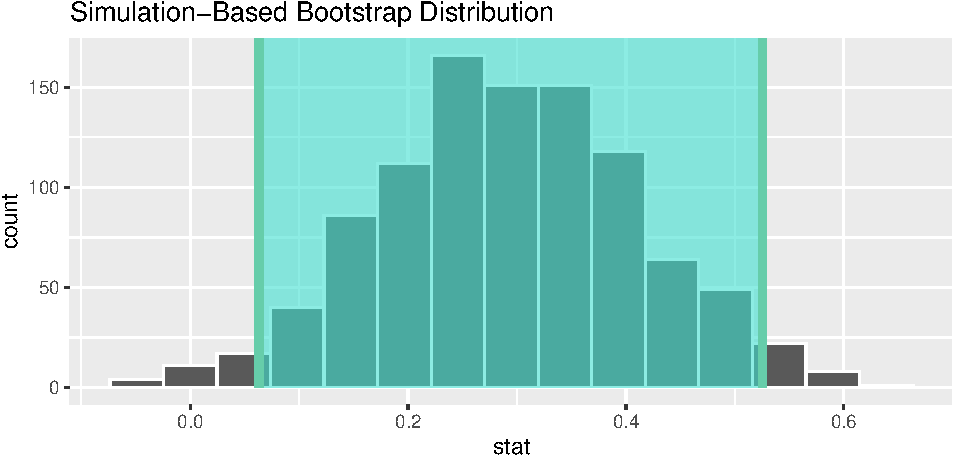
\includegraphics{tecnicas-cuantitativas_files/figure-latex/bootstrap-distribution-two-prop-percentile-1.pdf}
\caption{\label{fig:bootstrap-distribution-two-prop-percentile}Percentile-based 95\% confidence interval.}
\end{figure}

Notice a key value that is not included in the 95\% confidence interval for \(p_{m} - p_{f}\): the value 0. In other words, a difference of 0 is not included in our net, suggesting that \(p_{m}\) and \(p_{f}\) are truly different! Furthermore, observe how the entirety of the 95\% confidence interval for \(p_{m} - p_{f}\) lies above 0, suggesting that this difference is in favor of men.

Since the bootstrap distribution appears to be roughly normally shaped, we can also use the standard error method as we did in Section \ref{bootstrap-process}. In this case, we must specify the \texttt{point\_estimate} argument as the observed difference in promotion rates 0.292 = 29.2\% saved in \texttt{obs\_diff\_prop}. This value acts as the center of the confidence interval.

\begin{Shaded}
\begin{Highlighting}[]
\NormalTok{se_ci <-}\StringTok{ }\NormalTok{bootstrap_distribution }\OperatorTok\StringTok{ }
\StringTok{  }\KeywordTok{get_confidence_interval}\NormalTok{(}\DataTypeTok{level =} \FloatTok{0.95}\NormalTok{, }\DataTypeTok{type =} \StringTok{"se"}\NormalTok{, }
                          \DataTypeTok{point_estimate =}\NormalTok{ obs_diff_prop)}
\NormalTok{se_ci}
\end{Highlighting}
\end{Shaded}

\begin{verbatim}
## # A tibble: 1 x 2
##   lower_ci upper_ci
##      <dbl>    <dbl>
## 1   0.0587    0.525
\end{verbatim}

Let's visualize \texttt{bootstrap\_distribution} again, but now the standard error based 95\% confidence interval for \(p_{m} - p_{f}\) in Figure \ref{fig:bootstrap-distribution-two-prop-se}. Again, notice how the value 0 is not included in our confidence interval, again suggesting that \(p_{m}\) and \(p_{f}\) are truly different!

\begin{Shaded}
\begin{Highlighting}[]
\KeywordTok{visualize}\NormalTok{(bootstrap_distribution) }\OperatorTok{+}\StringTok{ }
\StringTok{  }\KeywordTok{shade_confidence_interval}\NormalTok{(}\DataTypeTok{endpoints =}\NormalTok{ se_ci)}
\end{Highlighting}
\end{Shaded}

\begin{figure}
\centering
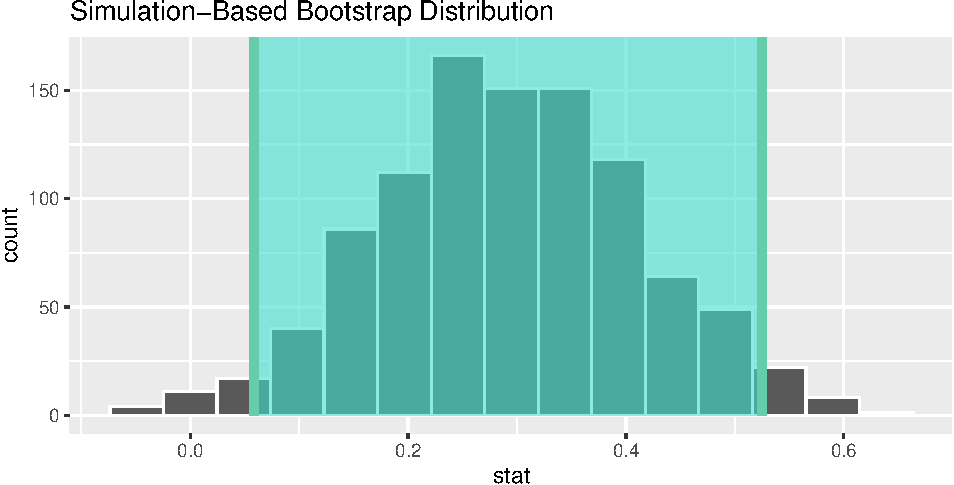
\includegraphics{tecnicas-cuantitativas_files/figure-latex/bootstrap-distribution-two-prop-se-1.pdf}
\caption{\label{fig:bootstrap-distribution-two-prop-se}Standard error-based 95\% confidence interval.}
\end{figure}

\hypertarget{only-one-test}{%
\subsection{``There is only one test''}\label{only-one-test}}

Let's recap the steps necessary to conduct a hypothesis test using the terminology, notation, and definitions related to sampling you saw in Section \ref{understanding-ht} and the \texttt{infer} workflow from Subsection \ref{infer-workflow-ht}:

\begin{enumerate}
\def\labelenumi{\arabic{enumi}.}
\tightlist
\item
  \texttt{specify()} the variables of interest in your data frame.
\item
  \texttt{hypothesize()} the null hypothesis \(H_0\). In other words, set a ``model for the universe'' assuming \(H_0\) is true.
\item
  \texttt{generate()} shuffles assuming \(H_0\) is true. In other words, \emph{simulate} data assuming \(H_0\) is true.
\item
  \texttt{calculate()} the \emph{test statistic} of interest, both for the observed data and your \emph{simulated} data.
\item
  \texttt{visualize()} the resulting \emph{null distribution} and compute the \emph{\(p\)-value} by comparing the null distribution to the observed test statistic.
\end{enumerate}

While this is a lot to digest, especially the first time you encounter hypothesis testing, the nice thing is that once you understand this general framework, then you can understand \emph{any} hypothesis test. In a famous blog post, computer scientist Allen Downey called this the \href{http://allendowney.blogspot.com/2016/06/there-is-still-only-one-test.html}{``There is only one test''} framework, for which he created the flowchart displayed in Figure \ref{fig:htdowney}.

Notice its similarity with the ``hypothesis testing with \texttt{infer}'' diagram you saw in Figure \ref{fig:inferht}. That's because the \texttt{infer} package was explicitly designed to match the ``There is only one test'' framework. So if you can understand the framework, you can easily generalize these ideas for all hypothesis testing scenarios. Whether for population proportions \(p\), population means \(\mu\), differences in population proportions \(p_1 - p_2\), differences in population means \(\mu_1 - \mu_2\), and as you'll see in Chapter \ref{inference-for-regression} on inference for regression, population regression slopes \(\beta_1\) as well. In fact, it applies more generally even than just these examples to more complicated hypothesis tests and test statistics as well.

\hypertarget{ht-interpretation}{%
\section{Interpreting hypothesis tests}\label{ht-interpretation}}

Interpreting the results of hypothesis tests is one of the more challenging aspects of this method for statistical inference. In this section, we'll focus on ways to help with deciphering the process and address some common misconceptions.

\hypertarget{trial}{%
\subsection{Two possible outcomes}\label{trial}}

In Section \ref{understanding-ht}, we mentioned that given a pre-specified significance level \(\alpha\) there are two possible outcomes of a hypothesis test:

\begin{itemize}
\tightlist
\item
  If the \(p\)-value is less than \(\alpha\), then we \emph{reject} the null hypothesis \(H_0\) in favor of \(H_A\).
\item
  If the \(p\)-value is greater than or equal to \(\alpha\), we \emph{fail to reject} the null hypothesis \(H_0\).
\end{itemize}

Unfortunately, the latter result is often misinterpreted as ``accepting the null hypothesis \(H_0\).'' While at first glance it may seem that the statements ``failing to reject \(H_0\)'' and ``accepting \(H_0\)'' are equivalent, there actually is a subtle difference. Saying that we ``accept the null hypothesis \(H_0\)'' is equivalent to stating that ``we think the null hypothesis \(H_0\) is true.'' However, saying that we ``fail to reject the null hypothesis \(H_0\)'' is saying something else: ``While \(H_0\) might still be false, we don't have enough evidence to say so.'' In other words, there is an absence of enough proof. However, the absence of proof is not proof of absence.

To further shed light on this distinction, \index{hypothesis testing!US criminal trial analogy} let's use the United States criminal justice system as an analogy. A criminal trial in the United States is a similar situation to hypothesis tests whereby a choice between two contradictory claims must be made about a defendant who is on trial:

\begin{enumerate}
\def\labelenumi{\arabic{enumi}.}
\tightlist
\item
  The defendant is truly either ``innocent'' or ``guilty.''
\item
  The defendant is presumed ``innocent until proven guilty.''
\item
  The defendant is found guilty only if there is \emph{strong evidence} that the defendant is guilty. The phrase ``beyond a reasonable doubt'' is often used as a guideline for determining a cutoff for when enough evidence exists to find the defendant guilty.
\item
  The defendant is found to be either ``not guilty'' or ``guilty'' in the ultimate verdict.
\end{enumerate}

In other words, \emph{not guilty} verdicts are not suggesting the defendant is \emph{innocent}, but instead that ``while the defendant may still actually be guilty, there wasn't enough evidence to prove this fact.'' Now let's make the connection with hypothesis tests:

\begin{enumerate}
\def\labelenumi{\arabic{enumi}.}
\tightlist
\item
  Either the null hypothesis \(H_0\) or the alternative hypothesis \(H_A\) is true.
\item
  Hypothesis tests are conducted assuming the null hypothesis \(H_0\) is true.
\item
  We reject the null hypothesis \(H_0\) in favor of \(H_A\) only if the evidence found in the sample suggests that \(H_A\) is true. The significance level \(\alpha\) is used as a guideline to set the threshold on just how strong of evidence we require.
\item
  We ultimately decide to either ``fail to reject \(H_0\)'' or ``reject \(H_0\).''
\end{enumerate}

So while gut instinct may suggest ``failing to reject \(H_0\)'' and ``accepting \(H_0\)'' are equivalent statements, they are not. ``Accepting \(H_0\)'' is equivalent to finding a defendant innocent. However, courts do not find defendants ``innocent,'' but rather they find them ``not guilty.'' Putting things differently, defense attorneys do not need to prove that their clients are innocent, rather they only need to prove that clients are not ``guilty beyond a reasonable doubt''.

So going back to our résumés activity in Section \ref{ht-infer}, recall that our hypothesis test was \(H_0: p_{m} - p_{f} = 0\) versus \(H_A: p_{m} - p_{f} > 0\) and that we used a pre-specified significance level of \(\alpha\) = 0.05. We found a \(p\)-value of 0.027. Since the \(p\)-value was smaller than \(\alpha\) = 0.05, we rejected \(H_0\). In other words, we found needed levels of evidence in this particular sample to say that \(H_0\) is false at the \(\alpha\) = 0.05 significance level. We also state this conclusion using non-statistical language: we found enough evidence in this data to suggest that there was gender discrimination at play.

\hypertarget{types-of-errors}{%
\subsection{Types of errors}\label{types-of-errors}}

Unfortunately, there is some chance a jury or a judge can make an incorrect decision in a criminal trial by reaching the wrong verdict. For example, finding a truly innocent defendant ``guilty''. Or on the other hand, finding a truly guilty defendant ``not guilty.'' This can often stem from the fact that prosecutors don't have access to all the relevant evidence, but instead are limited to whatever evidence the police can find.

The same holds for hypothesis tests. We can make incorrect decisions about a population parameter because we only have a sample of data from the population and thus sampling variation can lead us to incorrect conclusions.

There are two possible erroneous conclusions in a criminal trial: either (1) a truly innocent person is found guilty or (2) a truly guilty person is found not guilty. Similarly, there are two possible errors in a hypothesis test: either (1) rejecting \(H_0\) when in fact \(H_0\) is true, called a \textbf{Type I error} \index{hypothesis testing!Type I error} or (2) failing to reject \(H_0\) when in fact \(H_0\) is false, called a \index{hypothesis testing!Type II error} \textbf{Type II error}. Another term used for ``Type I error'' is ``false positive,'' while another term for ``Type II error'' is ``false negative.''

This risk of error is the price researchers pay for basing inference on a sample instead of performing a census on the entire population. But as we've seen in our numerous examples and activities so far, censuses are often very expensive and other times impossible, and thus researchers have no choice but to use a sample. Thus in any hypothesis test based on a sample, we have no choice but to tolerate some chance that a Type I error will be made and some chance that a Type II error will occur.

To help understand the concepts of Type I error and Type II errors, we apply these terms to our criminal justice analogy in Figure \ref{fig:trial-errors-table}.

Thus a Type I error corresponds to incorrectly putting a truly innocent person in jail, whereas a Type II error corresponds to letting a truly guilty person go free. Let's show the corresponding table in Figure \ref{fig:trial-errors-table-ht} for hypothesis tests.

\hypertarget{choosing-alpha}{%
\subsection{How do we choose alpha?}\label{choosing-alpha}}

If we are using a sample to make inferences about a population, we run the risk of making errors. For confidence intervals, a corresponding ``error'' would be constructing a confidence interval that does not contain the true value of the population parameter. For hypothesis tests, this would be making either a Type I or Type II error. Obviously, we want to minimize the probability of either error; we want a small probability of making an incorrect conclusion:

\begin{itemize}
\tightlist
\item
  The probability of a Type I Error occurring is denoted by \(\alpha\). The value of \(\alpha\) is called the \emph{significance level} of the hypothesis test, which we defined in Section \ref{understanding-ht}.
\item
  The probability of a Type II Error is denoted by \(\beta\). The value of \(1-\beta\) is known as the \emph{power} of the hypothesis test.
\end{itemize}

In other words, \(\alpha\) corresponds to the probability of incorrectly rejecting \(H_0\) when in fact \(H_0\) is true. On the other hand, \(\beta\) corresponds to the probability of incorrectly failing to reject \(H_0\) when in fact \(H_0\) is false.

Ideally, we want \(\alpha = 0\) and \(\beta = 0\), meaning that the chance of making either error is 0. However, this can never be the case in any situation where we are sampling for inference. There will always be the possibility of making either error when we use sample data. Furthermore, these two error probabilities are inversely related. As the probability of a Type I error goes down, the probability of a Type II error goes up.

What is typically done in practice is to fix the probability of a Type I error by pre-specifying a significance level \(\alpha\) and then try to minimize \(\beta\). In other words, we will tolerate a certain fraction of incorrect rejections of the null hypothesis \(H_0\), and then try to minimize the fraction of incorrect non-rejections of \(H_0\).

So for example if we used \(\alpha\) = 0.01, we would be using a hypothesis testing procedure that in the long run would incorrectly reject the null hypothesis \(H_0\) one percent of the time. This is analogous to setting the confidence level of a confidence interval.

So what value should you use for \(\alpha\)? \index{hypothesis testing!tradeoff between alpha and beta} Different fields have different conventions, but some commonly used values include 0.10, 0.05, 0.01, and 0.001. However, it is important to keep in mind that if you use a relatively small value of \(\alpha\), then all things being equal, \(p\)-values will have a harder time being less than \(\alpha\). Thus we would reject the null hypothesis less often. In other words, we would reject the null hypothesis \(H_0\) only if we have \emph{very strong} evidence to do so. This is known as a ``conservative'' test.

On the other hand, if we used a relatively large value of \(\alpha\), then all things being equal, \(p\)-values will have an easier time being less than \(\alpha\). Thus we would reject the null hypothesis more often. In other words, we would reject the null hypothesis \(H_0\) even if we only have \emph{mild} evidence to do so. This is known as a ``liberal'' test.

\hypertarget{conclusions}{%
\section{Conclusions}\label{conclusions}}

\hypertarget{when-inference-is-not-needed}{%
\subsection{When inference is not needed}\label{when-inference-is-not-needed}}

We've now walked through several different examples of how to use the \texttt{infer} package to perform statistical inference: constructing confidence intervals and conducting hypothesis tests. For each of these examples, we made it a point to always perform an exploratory data analysis (EDA) first; specifically, by looking at the raw data values, by using data visualization with \texttt{ggplot2}, and by data wrangling with \texttt{dplyr} beforehand. We \emph{highly} encourage you to always do the same. As a beginner to statistics, EDA helps you develop intuition as to what statistical methods like confidence intervals and hypothesis tests can tell us. Even as a seasoned practitioner of statistics, EDA helps guide your statistical investigations. In particular, is statistical inference even needed?

Let's consider an example. Say we're interested in the following question: Of \emph{all} flights leaving a New York City airport, are Hawaiian Airlines flights in the air for longer than Alaska Airlines flights? Furthermore, let's assume that 2013 flights are a representative sample of all such flights. Then we can use the \texttt{flights} data frame in the \texttt{nycflights13} \index{R packages!nycflights13} package we introduced in Section \ref{nycflights13} to answer our question. Let's filter this data frame to only include Hawaiian and Alaska Airlines using their \texttt{carrier} codes \texttt{HA} and \texttt{AS}:

\begin{Shaded}
\begin{Highlighting}[]
\NormalTok{flights_sample <-}\StringTok{ }\NormalTok{flights }\OperatorTok\StringTok{ }
\StringTok{  }\KeywordTok{filter}\NormalTok{(carrier }\OperatorTok\StringTok{ }\KeywordTok{c}\NormalTok{(}\StringTok{"HA"}\NormalTok{, }\StringTok{"AS"}\NormalTok{))}
\end{Highlighting}
\end{Shaded}

There are two possible statistical inference methods we could use to answer such questions. First, we could construct a 95\% confidence interval for the difference in population means \(\mu_{HA} - \mu_{AS}\), where \(\mu_{HA}\) is the mean air time of all Hawaiian Airlines flights and \(\mu_{AS}\) is the mean air time of all Alaska Airlines flights. We could then check if the entirety of the interval is greater than 0, suggesting that \(\mu_{HA} - \mu_{AS} > 0\), or, in other words suggesting that \(\mu_{HA} > \mu_{AS}\). Second, we could perform a hypothesis test of the null hypothesis \(H_0: \mu_{HA} - \mu_{AS} = 0\) versus the alternative hypothesis \(H_A: \mu_{HA} - \mu_{AS} > 0\).

However, let's first construct an exploratory visualization as we suggested earlier. Since \texttt{air\_time} is numerical and \texttt{carrier} is categorical, a boxplot can display the relationship between these two variables, which we display in Figure \ref{fig:ha-as-flights-boxplot}.

\begin{Shaded}
\begin{Highlighting}[]
\KeywordTok{ggplot}\NormalTok{(}\DataTypeTok{data =}\NormalTok{ flights_sample, }\DataTypeTok{mapping =} \KeywordTok{aes}\NormalTok{(}\DataTypeTok{x =}\NormalTok{ carrier, }\DataTypeTok{y =}\NormalTok{ air_time)) }\OperatorTok{+}
\StringTok{  }\KeywordTok{geom_boxplot}\NormalTok{() }\OperatorTok{+}
\StringTok{  }\KeywordTok{labs}\NormalTok{(}\DataTypeTok{x =} \StringTok{"Carrier"}\NormalTok{, }\DataTypeTok{y =} \StringTok{"Air Time"}\NormalTok{)}
\end{Highlighting}
\end{Shaded}

\begin{verbatim}
## Warning: Removed 5 rows containing non-finite values (stat_boxplot).
\end{verbatim}

\begin{figure}
\centering
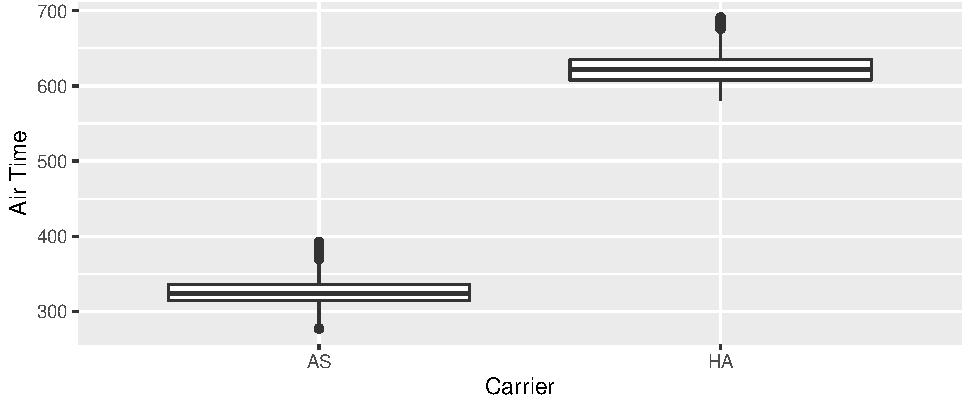
\includegraphics{tecnicas-cuantitativas_files/figure-latex/ha-as-flights-boxplot-1.pdf}
\caption{\label{fig:ha-as-flights-boxplot}Air time for Hawaiian and Alaska Airlines flights departing NYC in 2013.}
\end{figure}

This is what we like to call ``no PhD in Statistics needed'' moments. You don't have to be an expert in statistics to know that Alaska Airlines and Hawaiian Airlines have \emph{significantly} different air times. The two boxplots don't even overlap! Constructing a confidence interval or conducting a hypothesis test would frankly not provide much more insight than Figure \ref{fig:ha-as-flights-boxplot}.

Let's investigate why we observe such a clear cut difference between these two airlines using data wrangling. Let's first group by the rows of \texttt{flights\_sample} not only by \texttt{carrier} but also by destination \texttt{dest}. Subsequently, we'll compute two summary statistics: the number of observations using \texttt{n()} and the mean airtime:

\begin{Shaded}
\begin{Highlighting}[]
\NormalTok{flights_sample }\OperatorTok\StringTok{ }
\StringTok{  }\KeywordTok{group_by}\NormalTok{(carrier, dest) }\OperatorTok\StringTok{ }
\StringTok{  }\KeywordTok{summarize}\NormalTok{(}\DataTypeTok{n =} \KeywordTok{n}\NormalTok{(), }\DataTypeTok{mean_time =} \KeywordTok{mean}\NormalTok{(air_time, }\DataTypeTok{na.rm =} \OtherTok{TRUE}\NormalTok{))}
\end{Highlighting}
\end{Shaded}

\begin{verbatim}
## `summarise()` regrouping output by 'carrier' (override with `.groups` argument)
\end{verbatim}

\begin{verbatim}
## # A tibble: 2 x 4
## # Groups:   carrier [2]
##   carrier dest      n mean_time
##   <chr>   <chr> <int>     <dbl>
## 1 AS      SEA     714      326.
## 2 HA      HNL     342      623.
\end{verbatim}

It turns out that from New York City in 2013, Alaska only flew to \texttt{SEA} (Seattle) from New York City (NYC) while Hawaiian only flew to \texttt{HNL} (Honolulu) from NYC. Given the clear difference in distance from New York City to Seattle versus New York City to Honolulu, it is not surprising that we observe such different (\emph{statistically significantly different}, in fact) air times in flights.

This is a clear example of not needing to do anything more than a simple exploratory data analysis using data visualization and descriptive statistics to get an appropriate conclusion. This is why we highly recommend you perform an EDA of any sample data before running statistical inference methods like confidence intervals and hypothesis tests.

\hypertarget{problems-with-p-values}{%
\subsection{Problems with p-values}\label{problems-with-p-values}}

On top of the many common misunderstandings about hypothesis testing and \(p\)-values we listed in Section \ref{ht-interpretation}, another unfortunate consequence of the expanded use of \(p\)-values and hypothesis testing is a phenomenon known as ``p-hacking.'' \index{p-hacking} p-hacking is the act of ``cherry-picking'' only results that are ``statistically significant'' while dismissing those that aren't, even if at the expense of the scientific ideas. There are lots of articles written recently about misunderstandings and the problems with \(p\)-values. We encourage you to check some of them out:

\begin{enumerate}
\def\labelenumi{\arabic{enumi}.}
\tightlist
\item
  \href{https://en.wikipedia.org/wiki/Misunderstandings_of_p-values}{Misunderstandings of \(p\)-values}
\item
  \href{https://www.vox.com/science-and-health/2017/7/31/16021654/p-values-statistical-significance-redefine-0005}{What a nerdy debate about \(p\)-values shows about science - and how to fix it}
\item
  \href{https://www.nature.com/news/statisticians-issue-warning-over-misuse-of-p-values-1.19503}{Statisticians issue warning over misuse of \(P\) values}
\item
  \href{https://fivethirtyeight.com/features/you-cant-trust-what-you-read-about-nutrition/}{You Can't Trust What You Read About Nutrition}
\item
  \href{http://www.fharrell.com/post/pval-litany/}{A Litany of Problems with p-values}
\end{enumerate}

Such issues were getting so problematic that the American Statistical Association (ASA) put out a statement in 2016 titled, \href{https://www.amstat.org/asa/files/pdfs/P-ValueStatement.pdf}{``The ASA Statement on Statistical Significance and \(P\)-Values,''} with six principles underlying the proper use and interpretation of \(p\)-values. The ASA released this guidance on \(p\)-values to improve the conduct and interpretation of quantitative science and to inform the growing emphasis on reproducibility of science research.

We as authors much prefer the use of confidence intervals for statistical inference, since in our opinion they are much less prone to large misinterpretation. However, many fields still exclusively use \(p\)-values for statistical inference and this is one reason for including them in this text. We encourage you to learn more about ``p-hacking'' as well and its implication for science.

\hypertarget{el-muestreo-estaduxedstico}{%
\chapter{El muestreo estadístico}\label{el-muestreo-estaduxedstico}}

Some \emph{significant} applications are demonstrated in this chapter.

\hypertarget{example-one}{%
\section{Example one}\label{example-one}}

\hypertarget{example-two}{%
\section{Example two}\label{example-two}}

\hypertarget{regresiones}{%
\chapter{Regresiones}\label{regresiones}}

We have finished a nice book.

\hypertarget{estaduxedstica-multivariante}{%
\chapter{Estadística multivariante}\label{estaduxedstica-multivariante}}

We have finished a nice book.

  \bibliography{book.bib,packages.bib}

\end{document}
